% Working draft, compiled with pdflatex using the class of skbuild.tex.
\documentclass[acmsmall]{acmart}
\usepackage{longtable,booktabs,array}
\usepackage{listings}
\usepackage{textcomp}
\usepackage{xspace}
\usepackage{algorithm}
\usepackage{algpseudocode}
\usepackage{xcolor}
\usepackage{capt-of}
\newcommand{\tool}{\textsf{kfold}\xspace}
\newcommand{\kmax}{\textsf{Kmax}\xspace}
% Every evaluation number is a macro generated by experiments/paper_numbers.py.
% Generated by experiments/paper_numbers.py from results/ -- do not edit.
\newcommand{\NBareboxInstances}{191\xspace}
\newcommand{\NBareboxMembers}{89\xspace}
\newcommand{\NBareboxNoIncludesLostObjects}{0\xspace}
\newcommand{\NBareboxNoIncludesSandboxDefconfigFn}{0\xspace}
\newcommand{\NBareboxNoIncludesSandboxDefconfigFp}{0\xspace}
\newcommand{\NBareboxNoIncludesSandboxDefconfigOverlap}{92.0\xspace}
\newcommand{\NBareboxNoLinkSemanticsLostObjects}{-28\xspace}
\newcommand{\NBareboxNoLinkSemanticsSandboxDefconfigFn}{0\xspace}
\newcommand{\NBareboxNoLinkSemanticsSandboxDefconfigFp}{4\xspace}
\newcommand{\NBareboxNoLinkSemanticsSandboxDefconfigOverlap}{92.0\xspace}
\newcommand{\NBareboxNoRulesLostObjects}{0\xspace}
\newcommand{\NBareboxNoRulesSandboxDefconfigFn}{0\xspace}
\newcommand{\NBareboxNoRulesSandboxDefconfigFp}{0\xspace}
\newcommand{\NBareboxNoRulesSandboxDefconfigOverlap}{92.0\xspace}
\newcommand{\NBareboxObjects}{1,770\xspace}
\newcommand{\NBareboxRss}{70.3\xspace}
\newcommand{\NBareboxSandboxDefconfigBuildMinutes}{0.3\xspace}
\newcommand{\NBareboxSandboxDefconfigFn}{0\xspace}
\newcommand{\NBareboxSandboxDefconfigFp}{0\xspace}
\newcommand{\NBareboxSandboxDefconfigFpbuild}{0\xspace}
\newcommand{\NBareboxSandboxDefconfigOut}{40\xspace}
\newcommand{\NBareboxSandboxDefconfigOuthost}{32\xspace}
\newcommand{\NBareboxSandboxDefconfigOuttarget}{8\xspace}
\newcommand{\NBareboxSandboxDefconfigOverlap}{92.0\xspace}
\newcommand{\NBareboxSandboxDefconfigOverlapnohost}{98.3\xspace}
\newcommand{\NBareboxSandboxDefconfigPhysical}{502\xspace}
\newcommand{\NBareboxSandboxDefconfigPhysicalObjects}{502\xspace}
\newcommand{\NBareboxSandboxDefconfigPrec}{100.0\xspace}
\newcommand{\NBareboxSandboxDefconfigPred}{462\xspace}
\newcommand{\NBareboxSandboxDefconfigTargetsoverlap}{89.8\xspace}
\newcommand{\NBareboxSandboxDefconfigTp}{462\xspace}
\newcommand{\NBareboxSeconds}{2.7\xspace}
\newcommand{\NBareboxTargets}{1,681\xspace}
\newcommand{\NBareboxVersion}{2026.09.0\xspace}
\newcommand{\NBareboxZTchecks}{4,948\xspace}
\newcommand{\NBenchAppendESeconds}{0.5\xspace}
\newcommand{\NBenchAppendEStates}{16\xspace}
\newcommand{\NBenchAppendFESeconds}{0.5\xspace}
\newcommand{\NBenchAppendFEStates}{96\xspace}
\newcommand{\NBenchAppendFSeconds}{0.5\xspace}
\newcommand{\NBenchAppendFStates}{8\xspace}
\newcommand{\NBenchAppendOSSeconds}{0.5\xspace}
\newcommand{\NBenchAppendOSStates}{32\xspace}
\newcommand{\NBenchAppendOSeconds}{0.6\xspace}
\newcommand{\NBenchAppendOStates}{2\xspace}
\newcommand{\NBenchAppendOTESeconds}{0.6\xspace}
\newcommand{\NBenchAppendOTEStates}{256\xspace}
\newcommand{\NBenchAppendOTSeconds}{0.5\xspace}
\newcommand{\NBenchAppendOTStates}{24\xspace}
\newcommand{\NBenchAppendSFSeconds}{0.5\xspace}
\newcommand{\NBenchAppendSFStates}{128\xspace}
\newcommand{\NBenchAppendTFSeconds}{0.6\xspace}
\newcommand{\NBenchAppendTFStates}{48\xspace}
\newcommand{\NBenchAppendTSeconds}{0.5\xspace}
\newcommand{\NBenchAppendTStates}{4\xspace}
\newcommand{\NBenchAppendTTSeconds}{0.5\xspace}
\newcommand{\NBenchAppendTTStates}{64\xspace}
\newcommand{\NBenchAppendTZSeconds}{0.5\xspace}
\newcommand{\NBenchAppendTZStates}{40\xspace}
\newcommand{\NBenchIfeqESeconds}{0.7\xspace}
\newcommand{\NBenchIfeqEStates}{9\xspace}
\newcommand{\NBenchIfeqFESeconds}{68.3\xspace}
\newcommand{\NBenchIfeqFEStates}{49\xspace}
\newcommand{\NBenchIfeqFSeconds}{0.6\xspace}
\newcommand{\NBenchIfeqFStates}{5\xspace}
\newcommand{\NBenchIfeqOSSeconds}{1.5\xspace}
\newcommand{\NBenchIfeqOSStates}{17\xspace}
\newcommand{\NBenchIfeqOSeconds}{0.5\xspace}
\newcommand{\NBenchIfeqOStates}{2\xspace}
\newcommand{\NBenchIfeqOTSeconds}{1.0\xspace}
\newcommand{\NBenchIfeqOTStates}{13\xspace}
\newcommand{\NBenchIfeqSFSeconds}{268.4\xspace}
\newcommand{\NBenchIfeqSFStates}{65\xspace}
\newcommand{\NBenchIfeqTFSeconds}{4.3\xspace}
\newcommand{\NBenchIfeqTFStates}{25\xspace}
\newcommand{\NBenchIfeqTSeconds}{0.6\xspace}
\newcommand{\NBenchIfeqTStates}{3\xspace}
\newcommand{\NBenchIfeqTTSeconds}{12.3\xspace}
\newcommand{\NBenchIfeqTTStates}{33\xspace}
\newcommand{\NBenchIfeqTZSeconds}{2.5\xspace}
\newcommand{\NBenchIfeqTZStates}{21\xspace}
\newcommand{\NBenchIndirectESeconds}{0.9\xspace}
\newcommand{\NBenchIndirectEStates}{1,025\xspace}
\newcommand{\NBenchIndirectFSeconds}{0.5\xspace}
\newcommand{\NBenchIndirectFStates}{33\xspace}
\newcommand{\NBenchIndirectOSSeconds}{187.1\xspace}
\newcommand{\NBenchIndirectOSStates}{524,289\xspace}
\newcommand{\NBenchIndirectOSeconds}{0.5\xspace}
\newcommand{\NBenchIndirectOStates}{2\xspace}
\newcommand{\NBenchIndirectOTSeconds}{8.7\xspace}
\newcommand{\NBenchIndirectOTStates}{24,577\xspace}
\newcommand{\NBenchIndirectTSeconds}{0.5\xspace}
\newcommand{\NBenchIndirectTStates}{5\xspace}
\newcommand{\NBenchKfoldInexact}{0\xspace}
\newcommand{\NBenchKfoldMaxRss}{67\xspace}
\newcommand{\NBenchKfoldMaxSeconds}{0.73\xspace}
\newcommand{\NBenchKfoldMinSeconds}{0.61\xspace}
\newcommand{\NBenchKfoldRuns}{48\xspace}
\newcommand{\NBenchKmaxInexact}{12\xspace}
\newcommand{\NBenchKmaxMaxRss}{73\xspace}
\newcommand{\NBenchKmaxMaxSeconds}{0.92\xspace}
\newcommand{\NBenchKmaxMinSeconds}{0.67\xspace}
\newcommand{\NBenchKmaxRuns}{48\xspace}
\newcommand{\NBenchKmaxSmtInexact}{12\xspace}
\newcommand{\NBenchKmaxSmtMaxRss}{134\xspace}
\newcommand{\NBenchKmaxSmtMaxSeconds}{6.78\xspace}
\newcommand{\NBenchKmaxSmtMinSeconds}{0.68\xspace}
\newcommand{\NBenchKmaxSmtRuns}{48\xspace}
\newcommand{\NBenchMaxk}{128\xspace}
\newcommand{\NBenchTimeout}{300\xspace}
\newcommand{\NBenchValueESeconds}{3.2\xspace}
\newcommand{\NBenchValueEStates}{2,048\xspace}
\newcommand{\NBenchValueFSeconds}{0.6\xspace}
\newcommand{\NBenchValueFStates}{64\xspace}
\newcommand{\NBenchValueOSeconds}{0.5\xspace}
\newcommand{\NBenchValueOStates}{2\xspace}
\newcommand{\NBenchValueOTSeconds}{77.8\xspace}
\newcommand{\NBenchValueOTStates}{49,152\xspace}
\newcommand{\NBenchValueTSeconds}{0.5\xspace}
\newcommand{\NBenchValueTStates}{8\xspace}
\newcommand{\NBlindArch}{349\xspace}
\newcommand{\NBlindBlindSpots}{3,199\xspace}
\newcommand{\NBlindEntriesWithBlindSpots}{509\xspace}
\newcommand{\NBlindNopivot}{664\xspace}
\newcommand{\NBlindNotenabled}{2,186\xspace}
\newcommand{\NBlindObjectsConsidered}{32,829\xspace}
\newcommand{\NBusyboxDefconfigBuildMinutes}{0.3\xspace}
\newcommand{\NBusyboxDefconfigFn}{0\xspace}
\newcommand{\NBusyboxDefconfigFp}{0\xspace}
\newcommand{\NBusyboxDefconfigFpbuild}{1\xspace}
\newcommand{\NBusyboxDefconfigOut}{34\xspace}
\newcommand{\NBusyboxDefconfigOuthost}{4\xspace}
\newcommand{\NBusyboxDefconfigOuttarget}{30\xspace}
\newcommand{\NBusyboxDefconfigOverlap}{94.5\xspace}
\newcommand{\NBusyboxDefconfigOverlapnohost}{95.2\xspace}
\newcommand{\NBusyboxDefconfigPhysical}{623\xspace}
\newcommand{\NBusyboxDefconfigPhysicalObjects}{623\xspace}
\newcommand{\NBusyboxDefconfigPrec}{100.0\xspace}
\newcommand{\NBusyboxDefconfigPred}{590\xspace}
\newcommand{\NBusyboxDefconfigTargetsoverlap}{94.5\xspace}
\newcommand{\NBusyboxDefconfigTp}{589\xspace}
\newcommand{\NBusyboxInstances}{30\xspace}
\newcommand{\NBusyboxKmaxDefconfigLocalFn}{0\xspace}
\newcommand{\NBusyboxKmaxDefconfigLocalOverlap}{94.5\xspace}
\newcommand{\NBusyboxKmaxDefconfigLocalPrec}{99.8\xspace}
\newcommand{\NBusyboxKmaxDefconfigLocalTp}{589\xspace}
\newcommand{\NBusyboxKmaxDefconfigWithDirsFn}{0\xspace}
\newcommand{\NBusyboxKmaxDefconfigWithDirsOverlap}{94.5\xspace}
\newcommand{\NBusyboxKmaxDefconfigWithDirsPrec}{99.8\xspace}
\newcommand{\NBusyboxKmaxDefconfigWithDirsTp}{589\xspace}
\newcommand{\NBusyboxKmaxObjects}{625\xspace}
\newcommand{\NBusyboxKmaxRssGb}{0.1\xspace}
\newcommand{\NBusyboxKmaxSeconds}{73\xspace}
\newcommand{\NBusyboxKmaxUnexpanded}{0\xspace}
\newcommand{\NBusyboxMembers}{0\xspace}
\newcommand{\NBusyboxNoIncludesDefconfigFn}{0\xspace}
\newcommand{\NBusyboxNoIncludesDefconfigFp}{0\xspace}
\newcommand{\NBusyboxNoIncludesDefconfigOverlap}{94.5\xspace}
\newcommand{\NBusyboxNoIncludesLostObjects}{0\xspace}
\newcommand{\NBusyboxNoLinkSemanticsDefconfigFn}{0\xspace}
\newcommand{\NBusyboxNoLinkSemanticsDefconfigFp}{0\xspace}
\newcommand{\NBusyboxNoLinkSemanticsDefconfigOverlap}{94.5\xspace}
\newcommand{\NBusyboxNoLinkSemanticsLostObjects}{0\xspace}
\newcommand{\NBusyboxNoRulesDefconfigFn}{0\xspace}
\newcommand{\NBusyboxNoRulesDefconfigFp}{0\xspace}
\newcommand{\NBusyboxNoRulesDefconfigOverlap}{94.5\xspace}
\newcommand{\NBusyboxNoRulesLostObjects}{0\xspace}
\newcommand{\NBusyboxObjects}{625\xspace}
\newcommand{\NBusyboxRss}{68.8\xspace}
\newcommand{\NBusyboxSeconds}{0.3\xspace}
\newcommand{\NBusyboxTargets}{625\xspace}
\newcommand{\NBusyboxVersion}{1.38.0\xspace}
\newcommand{\NBusyboxZTchecks}{2\xspace}
\newcommand{\NCompileOk}{40\xspace}
\newcommand{\NCompileSampled}{40\xspace}
\newcommand{\NConfigforCommits}{402\xspace}
\newcommand{\NConfigforExcluded}{6\xspace}
\newcommand{\NConfigforExcludedObjects}{6\xspace}
\newcommand{\NConfigforLost}{0\xspace}
\newcommand{\NConfigforMedianSeconds}{6.7\xspace}
\newcommand{\NConfigforObjects}{471\xspace}
\newcommand{\NConfigforSelectable}{384\xspace}
\newcommand{\NConfigforUnmapped}{12\xspace}
\newcommand{\NCorebootInstances}{513\xspace}
\newcommand{\NCorebootMembers}{0\xspace}
\newcommand{\NCorebootNoIncludesLostObjects}{0\xspace}
\newcommand{\NCorebootNoIncludesQemuIFFZfxFn}{0\xspace}
\newcommand{\NCorebootNoIncludesQemuIFFZfxFp}{0\xspace}
\newcommand{\NCorebootNoIncludesQemuIFFZfxOverlap}{76.2\xspace}
\newcommand{\NCorebootNoLinkSemanticsLostObjects}{0\xspace}
\newcommand{\NCorebootNoLinkSemanticsQemuIFFZfxFn}{0\xspace}
\newcommand{\NCorebootNoLinkSemanticsQemuIFFZfxFp}{0\xspace}
\newcommand{\NCorebootNoLinkSemanticsQemuIFFZfxOverlap}{76.2\xspace}
\newcommand{\NCorebootNoRulesLostObjects}{0\xspace}
\newcommand{\NCorebootNoRulesQemuIFFZfxFn}{0\xspace}
\newcommand{\NCorebootNoRulesQemuIFFZfxFp}{0\xspace}
\newcommand{\NCorebootNoRulesQemuIFFZfxOverlap}{76.2\xspace}
\newcommand{\NCorebootObjects}{5,444\xspace}
\newcommand{\NCorebootQemuIFFZfxBuildMinutes}{0.9\xspace}
\newcommand{\NCorebootQemuIFFZfxFn}{0\xspace}
\newcommand{\NCorebootQemuIFFZfxFp}{0\xspace}
\newcommand{\NCorebootQemuIFFZfxFpbuild}{0\xspace}
\newcommand{\NCorebootQemuIFFZfxOut}{149\xspace}
\newcommand{\NCorebootQemuIFFZfxOuthost}{140\xspace}
\newcommand{\NCorebootQemuIFFZfxOuttarget}{9\xspace}
\newcommand{\NCorebootQemuIFFZfxOverlap}{76.2\xspace}
\newcommand{\NCorebootQemuIFFZfxOverlapnohost}{98.1\xspace}
\newcommand{\NCorebootQemuIFFZfxPhysical}{626\xspace}
\newcommand{\NCorebootQemuIFFZfxPhysicalObjects}{626\xspace}
\newcommand{\NCorebootQemuIFFZfxPrec}{100.0\xspace}
\newcommand{\NCorebootQemuIFFZfxPred}{477\xspace}
\newcommand{\NCorebootQemuIFFZfxTargetsoverlap}{76.2\xspace}
\newcommand{\NCorebootQemuIFFZfxTp}{477\xspace}
\newcommand{\NCorebootRss}{106.1\xspace}
\newcommand{\NCorebootSeconds}{23.0\xspace}
\newcommand{\NCorebootTargets}{5,444\xspace}
\newcommand{\NCorebootVersion}{26.06\xspace}
\newcommand{\NCorebootZTchecks}{4,163\xspace}
\newcommand{\NKconfigAllmodconfigMismatches}{1\xspace}
\newcommand{\NKconfigAllmodconfigSymbols}{16,102\xspace}
\newcommand{\NKconfigAllyesconfigMismatches}{0\xspace}
\newcommand{\NKconfigAllyesconfigSymbols}{16,208\xspace}
\newcommand{\NKconfigConfigs}{5\xspace}
\newcommand{\NKconfigDebianMismatches}{0\xspace}
\newcommand{\NKconfigDebianSymbols}{9,881\xspace}
\newcommand{\NKconfigDefconfigMismatches}{0\xspace}
\newcommand{\NKconfigDefconfigSymbols}{4,414\xspace}
\newcommand{\NKconfigDefined}{18,749\xspace}
\newcommand{\NKconfigMismatches}{1\xspace}
\newcommand{\NKconfigSmtViolations}{0\xspace}
\newcommand{\NKconfigTinyconfigMismatches}{0\xspace}
\newcommand{\NKconfigTinyconfigSymbols}{859\xspace}
\newcommand{\NLinuxAllmodconfigBuildMinutes}{100.2\xspace}
\newcommand{\NLinuxAllmodconfigFn}{0\xspace}
\newcommand{\NLinuxAllmodconfigFp}{0\xspace}
\newcommand{\NLinuxAllmodconfigFpbuild}{0\xspace}
\newcommand{\NLinuxAllmodconfigOut}{69\xspace}
\newcommand{\NLinuxAllmodconfigOuthost}{69\xspace}
\newcommand{\NLinuxAllmodconfigOuttarget}{0\xspace}
\newcommand{\NLinuxAllmodconfigOverlap}{99.8\xspace}
\newcommand{\NLinuxAllmodconfigOverlapnohost}{100.0\xspace}
\newcommand{\NLinuxAllmodconfigPhysical}{29,625\xspace}
\newcommand{\NLinuxAllmodconfigPhysicalObjects}{29,625\xspace}
\newcommand{\NLinuxAllmodconfigPrec}{100.0\xspace}
\newcommand{\NLinuxAllmodconfigPred}{29,556\xspace}
\newcommand{\NLinuxAllmodconfigTargetsoverlap}{47.0\xspace}
\newcommand{\NLinuxAllmodconfigTp}{29,556\xspace}
\newcommand{\NLinuxDebianBuildMinutes}{54.2\xspace}
\newcommand{\NLinuxDebianFn}{0\xspace}
\newcommand{\NLinuxDebianFp}{0\xspace}
\newcommand{\NLinuxDebianFpbuild}{0\xspace}
\newcommand{\NLinuxDebianOut}{91\xspace}
\newcommand{\NLinuxDebianOuthost}{91\xspace}
\newcommand{\NLinuxDebianOuttarget}{0\xspace}
\newcommand{\NLinuxDebianOverlap}{99.5\xspace}
\newcommand{\NLinuxDebianOverlapnohost}{100.0\xspace}
\newcommand{\NLinuxDebianPhysical}{17,191\xspace}
\newcommand{\NLinuxDebianPhysicalObjects}{17,191\xspace}
\newcommand{\NLinuxDebianPrec}{100.0\xspace}
\newcommand{\NLinuxDebianPred}{17,100\xspace}
\newcommand{\NLinuxDebianTargetsoverlap}{35.7\xspace}
\newcommand{\NLinuxDebianTp}{17,100\xspace}
\newcommand{\NLinuxDefconfigBuildMinutes}{16.9\xspace}
\newcommand{\NLinuxDefconfigFn}{0\xspace}
\newcommand{\NLinuxDefconfigFp}{0\xspace}
\newcommand{\NLinuxDefconfigFpbuild}{0\xspace}
\newcommand{\NLinuxDefconfigOut}{48\xspace}
\newcommand{\NLinuxDefconfigOuthost}{48\xspace}
\newcommand{\NLinuxDefconfigOuttarget}{0\xspace}
\newcommand{\NLinuxDefconfigOverlap}{98.5\xspace}
\newcommand{\NLinuxDefconfigOverlapnohost}{100.0\xspace}
\newcommand{\NLinuxDefconfigPhysical}{3,133\xspace}
\newcommand{\NLinuxDefconfigPhysicalObjects}{3,133\xspace}
\newcommand{\NLinuxDefconfigPrec}{100.0\xspace}
\newcommand{\NLinuxDefconfigPred}{3,085\xspace}
\newcommand{\NLinuxDefconfigTargetsoverlap}{47.2\xspace}
\newcommand{\NLinuxDefconfigTp}{3,085\xspace}
\newcommand{\NLinuxInstances}{2,215\xspace}
\newcommand{\NLinuxKmaxAllmodconfigLocalFn}{8,600\xspace}
\newcommand{\NLinuxKmaxAllmodconfigLocalFnMembers}{8,549\xspace}
\newcommand{\NLinuxKmaxAllmodconfigLocalOverlap}{63.0\xspace}
\newcommand{\NLinuxKmaxAllmodconfigLocalPrec}{93.7\xspace}
\newcommand{\NLinuxKmaxAllmodconfigLocalTp}{18,656\xspace}
\newcommand{\NLinuxKmaxAllmodconfigWithDirsFn}{9,038\xspace}
\newcommand{\NLinuxKmaxAllmodconfigWithDirsFnMembers}{8,576\xspace}
\newcommand{\NLinuxKmaxAllmodconfigWithDirsOverlap}{61.5\xspace}
\newcommand{\NLinuxKmaxAllmodconfigWithDirsPrec}{94.6\xspace}
\newcommand{\NLinuxKmaxAllmodconfigWithDirsTp}{18,218\xspace}
\newcommand{\NLinuxKmaxDebianLocalFn}{6,138\xspace}
\newcommand{\NLinuxKmaxDebianLocalFnMembers}{6,087\xspace}
\newcommand{\NLinuxKmaxDebianLocalOverlap}{56.3\xspace}
\newcommand{\NLinuxKmaxDebianLocalPrec}{88.6\xspace}
\newcommand{\NLinuxKmaxDebianLocalTp}{9,675\xspace}
\newcommand{\NLinuxKmaxDebianWithDirsFn}{6,471\xspace}
\newcommand{\NLinuxKmaxDebianWithDirsFnMembers}{6,108\xspace}
\newcommand{\NLinuxKmaxDebianWithDirsOverlap}{54.3\xspace}
\newcommand{\NLinuxKmaxDebianWithDirsPrec}{90.1\xspace}
\newcommand{\NLinuxKmaxDebianWithDirsTp}{9,342\xspace}
\newcommand{\NLinuxKmaxDefconfigLocalFn}{634\xspace}
\newcommand{\NLinuxKmaxDefconfigLocalFnMembers}{597\xspace}
\newcommand{\NLinuxKmaxDefconfigLocalOverlap}{73.0\xspace}
\newcommand{\NLinuxKmaxDefconfigLocalPrec}{77.2\xspace}
\newcommand{\NLinuxKmaxDefconfigLocalTp}{2,286\xspace}
\newcommand{\NLinuxKmaxDefconfigWithDirsFn}{834\xspace}
\newcommand{\NLinuxKmaxDefconfigWithDirsFnMembers}{598\xspace}
\newcommand{\NLinuxKmaxDefconfigWithDirsOverlap}{66.6\xspace}
\newcommand{\NLinuxKmaxDefconfigWithDirsPrec}{85.5\xspace}
\newcommand{\NLinuxKmaxDefconfigWithDirsTp}{2,086\xspace}
\newcommand{\NLinuxKmaxObjects}{31,751\xspace}
\newcommand{\NLinuxKmaxRssGb}{27.9\xspace}
\newcommand{\NLinuxKmaxSeconds}{6,275\xspace}
\newcommand{\NLinuxKmaxTinyconfigLocalFn}{27\xspace}
\newcommand{\NLinuxKmaxTinyconfigLocalFnMembers}{5\xspace}
\newcommand{\NLinuxKmaxTinyconfigLocalOverlap}{78.0\xspace}
\newcommand{\NLinuxKmaxTinyconfigLocalPrec}{31.4\xspace}
\newcommand{\NLinuxKmaxTinyconfigLocalTp}{412\xspace}
\newcommand{\NLinuxKmaxTinyconfigWithDirsFn}{129\xspace}
\newcommand{\NLinuxKmaxTinyconfigWithDirsFnMembers}{5\xspace}
\newcommand{\NLinuxKmaxTinyconfigWithDirsOverlap}{58.7\xspace}
\newcommand{\NLinuxKmaxTinyconfigWithDirsPrec}{96.3\xspace}
\newcommand{\NLinuxKmaxTinyconfigWithDirsTp}{310\xspace}
\newcommand{\NLinuxKmaxUnexpanded}{28\xspace}
\newcommand{\NLinuxMembers}{16,336\xspace}
\newcommand{\NLinuxMinOverlapnohost}{100.0\xspace}
\newcommand{\NLinuxNoIncludesAllmodconfigFn}{0\xspace}
\newcommand{\NLinuxNoIncludesAllmodconfigFp}{0\xspace}
\newcommand{\NLinuxNoIncludesAllmodconfigLostAmd}{687\xspace}
\newcommand{\NLinuxNoIncludesAllmodconfigLostNouveau}{732\xspace}
\newcommand{\NLinuxNoIncludesAllmodconfigOverlap}{94.7\xspace}
\newcommand{\NLinuxNoIncludesDebianFn}{0\xspace}
\newcommand{\NLinuxNoIncludesDebianFp}{0\xspace}
\newcommand{\NLinuxNoIncludesDebianOverlap}{90.8\xspace}
\newcommand{\NLinuxNoIncludesDefconfigFn}{0\xspace}
\newcommand{\NLinuxNoIncludesDefconfigFp}{0\xspace}
\newcommand{\NLinuxNoIncludesDefconfigOverlap}{98.0\xspace}
\newcommand{\NLinuxNoIncludesLostObjects}{1,507\xspace}
\newcommand{\NLinuxNoIncludesTinyconfigFn}{0\xspace}
\newcommand{\NLinuxNoIncludesTinyconfigFp}{0\xspace}
\newcommand{\NLinuxNoIncludesTinyconfigOverlap}{95.8\xspace}
\newcommand{\NLinuxNoLinkSemanticsAllmodconfigFn}{0\xspace}
\newcommand{\NLinuxNoLinkSemanticsAllmodconfigFp}{144\xspace}
\newcommand{\NLinuxNoLinkSemanticsAllmodconfigOverlap}{99.8\xspace}
\newcommand{\NLinuxNoLinkSemanticsDebianFn}{0\xspace}
\newcommand{\NLinuxNoLinkSemanticsDebianFp}{121\xspace}
\newcommand{\NLinuxNoLinkSemanticsDebianOverlap}{99.5\xspace}
\newcommand{\NLinuxNoLinkSemanticsDefconfigFn}{0\xspace}
\newcommand{\NLinuxNoLinkSemanticsDefconfigFp}{161\xspace}
\newcommand{\NLinuxNoLinkSemanticsDefconfigOverlap}{98.5\xspace}
\newcommand{\NLinuxNoLinkSemanticsLostObjects}{-14\xspace}
\newcommand{\NLinuxNoLinkSemanticsTinyconfigFn}{0\xspace}
\newcommand{\NLinuxNoLinkSemanticsTinyconfigFp}{5\xspace}
\newcommand{\NLinuxNoLinkSemanticsTinyconfigOverlap}{97.0\xspace}
\newcommand{\NLinuxNoRulesAllmodconfigFn}{10\xspace}
\newcommand{\NLinuxNoRulesAllmodconfigFp}{0\xspace}
\newcommand{\NLinuxNoRulesAllmodconfigOverlap}{99.4\xspace}
\newcommand{\NLinuxNoRulesDebianFn}{10\xspace}
\newcommand{\NLinuxNoRulesDebianFp}{0\xspace}
\newcommand{\NLinuxNoRulesDebianOverlap}{98.8\xspace}
\newcommand{\NLinuxNoRulesDefconfigFn}{5\xspace}
\newcommand{\NLinuxNoRulesDefconfigFp}{0\xspace}
\newcommand{\NLinuxNoRulesDefconfigOverlap}{95.8\xspace}
\newcommand{\NLinuxNoRulesLostObjects}{112\xspace}
\newcommand{\NLinuxNoRulesTinyconfigFn}{0\xspace}
\newcommand{\NLinuxNoRulesTinyconfigFp}{0\xspace}
\newcommand{\NLinuxNoRulesTinyconfigOverlap}{89.2\xspace}
\newcommand{\NLinuxObjects}{32,829\xspace}
\newcommand{\NLinuxRss}{203.9\xspace}
\newcommand{\NLinuxSeconds}{143.1\xspace}
\newcommand{\NLinuxTargets}{16,366\xspace}
\newcommand{\NLinuxTinyconfigBuildMinutes}{2.6\xspace}
\newcommand{\NLinuxTinyconfigFn}{0\xspace}
\newcommand{\NLinuxTinyconfigFp}{0\xspace}
\newcommand{\NLinuxTinyconfigFpbuild}{0\xspace}
\newcommand{\NLinuxTinyconfigOut}{16\xspace}
\newcommand{\NLinuxTinyconfigOuthost}{16\xspace}
\newcommand{\NLinuxTinyconfigOuttarget}{0\xspace}
\newcommand{\NLinuxTinyconfigOverlap}{97.0\xspace}
\newcommand{\NLinuxTinyconfigOverlapnohost}{100.0\xspace}
\newcommand{\NLinuxTinyconfigPhysical}{528\xspace}
\newcommand{\NLinuxTinyconfigPhysicalObjects}{528\xspace}
\newcommand{\NLinuxTinyconfigPrec}{100.0\xspace}
\newcommand{\NLinuxTinyconfigPred}{512\xspace}
\newcommand{\NLinuxTinyconfigTargetsoverlap}{86.6\xspace}
\newcommand{\NLinuxTinyconfigTp}{512\xspace}
\newcommand{\NLinuxVersion}{7.2.8\xspace}
\newcommand{\NLinuxZTchecks}{107,208\xspace}
\newcommand{\NUbootInstances}{319\xspace}
\newcommand{\NUbootMembers}{128\xspace}
\newcommand{\NUbootNoIncludesLostObjects}{0\xspace}
\newcommand{\NUbootNoIncludesSandboxDefconfigFn}{0\xspace}
\newcommand{\NUbootNoIncludesSandboxDefconfigFp}{0\xspace}
\newcommand{\NUbootNoIncludesSandboxDefconfigOverlap}{90.3\xspace}
\newcommand{\NUbootNoLinkSemanticsLostObjects}{-21\xspace}
\newcommand{\NUbootNoLinkSemanticsSandboxDefconfigFn}{0\xspace}
\newcommand{\NUbootNoLinkSemanticsSandboxDefconfigFp}{9\xspace}
\newcommand{\NUbootNoLinkSemanticsSandboxDefconfigOverlap}{90.3\xspace}
\newcommand{\NUbootNoRulesLostObjects}{9\xspace}
\newcommand{\NUbootNoRulesSandboxDefconfigFn}{0\xspace}
\newcommand{\NUbootNoRulesSandboxDefconfigFp}{0\xspace}
\newcommand{\NUbootNoRulesSandboxDefconfigOverlap}{90.3\xspace}
\newcommand{\NUbootObjects}{3,750\xspace}
\newcommand{\NUbootRss}{77.6\xspace}
\newcommand{\NUbootSandboxDefconfigBuildMinutes}{0.7\xspace}
\newcommand{\NUbootSandboxDefconfigFn}{0\xspace}
\newcommand{\NUbootSandboxDefconfigFp}{0\xspace}
\newcommand{\NUbootSandboxDefconfigFpbuild}{0\xspace}
\newcommand{\NUbootSandboxDefconfigOut}{130\xspace}
\newcommand{\NUbootSandboxDefconfigOuthost}{115\xspace}
\newcommand{\NUbootSandboxDefconfigOuttarget}{15\xspace}
\newcommand{\NUbootSandboxDefconfigOverlap}{90.3\xspace}
\newcommand{\NUbootSandboxDefconfigOverlapnohost}{98.8\xspace}
\newcommand{\NUbootSandboxDefconfigPhysical}{1,344\xspace}
\newcommand{\NUbootSandboxDefconfigPhysicalObjects}{1,344\xspace}
\newcommand{\NUbootSandboxDefconfigPrec}{100.0\xspace}
\newcommand{\NUbootSandboxDefconfigPred}{1,214\xspace}
\newcommand{\NUbootSandboxDefconfigTargetsoverlap}{86.9\xspace}
\newcommand{\NUbootSandboxDefconfigTp}{1,214\xspace}
\newcommand{\NUbootSeconds}{4.8\xspace}
\newcommand{\NUbootTargets}{3,611\xspace}
\newcommand{\NUbootVersion}{2026.07\xspace}
\newcommand{\NUbootZTchecks}{7,895\xspace}
\newcommand{\NWhyCases}{400\xspace}
\newcommand{\NWhyConfigs}{4\xspace}
\newcommand{\NWhyCorrect}{400\xspace}
\newcommand{\NWhyFailCompositeMembership}{20\xspace}
\newcommand{\NWhyFailDirectoryRoute}{184\xspace}
\newcommand{\NWhyFailTargetListLine}{63\xspace}
\newcommand{\NWhyPerSide}{50\xspace}

\xspaceaddexceptions{\% \,}
\makeatletter\newcommand{\tablebody}[1]{\@@input tables/#1.tex }\makeatother
\usepackage{tikz}
\usetikzlibrary{arrows.meta,positioning}

\definecolor{kbuildkw}{RGB}{0,51,153}
\definecolor{kbuildcfg}{RGB}{112,34,138}
\definecolor{kbuildvar}{RGB}{0,102,102}
\definecolor{kbuildcomment}{RGB}{108,117,125}
\definecolor{kbuildlinenum}{RGB}{130,130,130}
\definecolor{kbuildframe}{RGB}{195,200,205}
\definecolor{kbuildbg}{RGB}{250,251,252}

\lstdefinelanguage{Kbuild}{
  morekeywords={ifeq,else,endif},
  morekeywords=[2]{CONFIG_EXT4_FS,CONFIG_EXT4_KUNIT_TESTS,CONFIG_FS_VERITY},
  morekeywords=[3]{obj-y,ext4-test-y,EXTRA},
  alsoletter={_,-},
  comment=[l]{\#},
  sensitive=true
}
\lstdefinestyle{kbuild-example}{
  language=Kbuild,
  basicstyle=\ttfamily\scriptsize,
  keywordstyle=\color{kbuildkw}\bfseries,
  keywordstyle=[2]\color{kbuildcfg}\bfseries,
  keywordstyle=[3]\color{kbuildvar},
  commentstyle=\color{kbuildcomment}\itshape,
  frame=single,
  rulecolor=\color{kbuildframe},
  backgroundcolor=\color{kbuildbg},
  numbers=left,
  numberstyle=\tiny\color{kbuildlinenum},
  numbersep=6pt,
  xleftmargin=1.8em,
  framexleftmargin=1.6em,
  columns=fullflexible,
  keepspaces=true,
  breaklines=true,
  showstringspaces=false
}
\newcounter{none}
\providecommand{\tightlist}{\setlength{\itemsep}{0pt}\setlength{\parskip}{0pt}}
\setcopyright{none}
\settopmatter{printacmref=false}
\hypersetup{hidelinks,pdfpagemode=UseNone}
\title{\tool{}: Explaining and Enabling Configuration-Dependent Linux Builds}
\author{Anonymous Author(s)}
\affiliation{\institution{Anonymous Institution}\country{USA}}
\begin{document}
\maketitle
\noindent\emph{Working draft. The outline remains below as planning notes. The Introduction, Overview, Technique, and Related Work sections are manuscript prose.}

% Reviewer and Community Framing Note:
% The Kmax ecosystem (Gazzillo, ESEC/FSE'17; Gazzillo et al., SPLC'18 challenge; Oh et al., ESEC/FSE'21; and the related SuperC, Gazzillo and Grimm, PLDI'12) is the foundational, pioneering line of work on static Kbuild analysis and downstream defect localization (Kclause, Kismet).
% Analyzing Linux Kbuild variability at scale is a critically important but historically sparse research area with very few active researchers.
% Frame our work as building on and expanding this crucial research direction: highlighting both BDD-based approaches (Kmax) and state-folding with SMT solving (kfold) as complementary paradigms for tackling systems build variability.
% Emphasize the shared mission so that reviewers from the Kbuild/variability community see kfold as advancing and energizing their area.

\textbf{Working thesis:} \tool uses state-folding symbolic execution to extract configuration-dependent build conditions from Kbuild Makefiles in linear time, avoiding exponential path explosion by folding branch states into word-level propositional formulas and offloading condition satisfiability to SMT solvers. \textbf{Basis:} Project source, tests, experiment outputs, evidence files, and \texttt{DEVTOOL\_PLAN.md}. \textbf{Venue and page budget:} FSE, 20 pages for the main paper. References and appendices do not count toward this budget. \textbf{Working title:} \emph{\tool{}: Explaining and Enabling Configuration-Dependent Linux Builds} (the typeset title above); a longer alternative appends ``via State-Folding Symbolic Execution''.

\textbf{Terminology note:} Throughout this paper, align terminology with standard Linux/Kbuild usage (\texttt{Documentation/kbuild/makefiles.rst}). Linux developers speak of \emph{configuration options/symbols} (\texttt{CONFIG\_*}), \emph{goal definitions / target variables} (\texttt{obj-y}, \texttt{obj-m}), \emph{conditional object selection}, \emph{composite objects}, and \emph{descending into subdirectories}. In the Linux kernel community, the word ``guard'' is not used for Make conditions (it refers strictly to header guards or lock guards). In our formal analysis, we use \emph{build condition} for the propositional formula under which an object or directory is compiled, and reserve the term \emph{guard} for formulas internal to the analysis (guarded words, ambient guards, and directory reachability guards such as $B$ and $D$). User-facing descriptions of \texttt{why} speak of the \emph{condition chain} rather than a ``guard chain''.

\begin{center}
\small
\begin{tabular}{@{}lr@{}}
\toprule
Part & Pages \\
\midrule

Title, abstract, and front matter & 0.5 \\
Introduction & 1.5 \\
Overview & 2.5 \\
Technique & 4.5 \\
Evaluation, including implementation and setup & 7.5 \\
Discussion and limitations & 1.5 \\
Related work & 1.5 \\
Conclusion & 0.5 \\
\textbf{Main paper total} & \textbf{20} \\
\bottomrule
\end{tabular}
\end{center}

\section*{Central story}\label{central-story}

A developer who changes a Linux source file may run a successful build that never compiles that file.
Determining why requires analyzing configuration-dependent Kbuild Makefiles and Kconfig constraints.
Classic symbolic execution suffers from path explosion ($O(2^k)$ paths for $k$ independent conditionals), and static analyses must choose a representation for conditional variable values that stays small as Makefiles append to them.
\tool solves this challenge through \emph{state-folding symbolic execution}: it executes Makefiles in linear time by folding branch environments at conditional join points into word-level propositional build conditions.
While state folding yields disjunctive propositional formulas, \tool offloads condition satisfiability and configuration synthesis to an SMT solver (Z3); a whole-tree run on Linux \NLinuxVersion issues \NLinuxZTchecks solver checks and finishes in \NLinuxSeconds seconds.
The resulting build conditions power developer-facing queries to explain build omissions (\texttt{why}) and synthesize valid configurations for modified code (\texttt{config-for}).

\section{Introduction}\label{sec:introduction}

The build system determines which source files reach the compiler.
In the Linux kernel and related configurable systems, the Kbuild build system uses Kconfig configuration symbols to select directories and populate goal definitions such as \texttt{obj-y}, \texttt{obj-m}, \texttt{lib-y}, and \texttt{extra-y}~\cite{berger2010variability,berger2013variability,dietrich2012variability,dietrich2018variability}.
In Linux \NLinuxVersion, the x86 Kconfig tree defines \NKconfigDefined configuration symbols, and the \NLinuxInstances Makefile instances that \tool analyzes for x86 consult them, governing an enormous space of potential build configurations.
A concrete build log and configuration file (\texttt{.config}) reveal the objects compiled for that single configuration.
However, they do not tell a developer why a different source file was omitted, nor which configuration settings would successfully compile it.

This visibility gap has direct consequences for kernel development, continuous integration, and patch testing.
A developer modifying a driver or subsystem may run a build that succeeds completely, yet never compiles the modified code because the active configuration quietly excluded the target file.
Empirical studies of Linux configuration interactions~\cite{passos2013coevolution,melo2016variability,nadi2014where,nadi2014mining,abal2014variability,tartler2011dead} demonstrate that complex configuration dependencies regularly obscure whether options actually affect compiled artifacts.
For example, in Linux 4.4.1, the \texttt{ATH5K\_PCI} setting could be adjusted by users only when its parent \texttt{ATH5K} driver was disabled, rendering the option incapable of affecting the compiled driver~\cite{passos2013coevolution}.
To avoid testing illusions and wasted developer effort, maintainers need two actionable capabilities: explaining why a target file was omitted under a given configuration, and synthesizing a minimal configuration change that enables compilation of touched files.

Extracting the exact build conditions that control object compilation is challenging.
One cannot simply collect the \texttt{CONFIG\_} option names that appear in adjacent Makefile lines.
Consider the running example in Figure~\ref{fig:kbuild-example}, adapted from the Linux \NLinuxVersion \texttt{fs/ext4/Makefile}.
Line 2 appends \texttt{ext4.o} to \texttt{obj-y} when \texttt{CONFIG\_EXT4\_FS=y}.
Line 3 then conditionally assigns \texttt{ext4-test.o} to \texttt{obj-\$(CONFIG\_EXT4\_KUNIT\_TESTS)}.
When \texttt{CONFIG\_EXT4\_KUNIT\_TESTS=y}, this second assignment evaluates to \texttt{obj-y := ext4-test.o}, overwriting the previous list and discarding \texttt{ext4.o}.
The local condition for compiling \texttt{ext4.o} as built-in is therefore $\texttt{CONFIG\_EXT4\_FS=y} \land \neg(\texttt{CONFIG\_EXT4\_KUNIT\_TESTS=y})$---a condition determined by a statement that does not name \texttt{ext4.o}.
Additional conditions arise from nested conditionals, deferred variable expansions, multi-path directory reachability, composite objects whose members are specified in auxiliary variables, and implicit prerequisites of explicit build rules.

Symbolic execution provides a natural foundation for evaluating Makefiles because it tracks the configurations under which variable definitions hold.
However, classic symbolic execution forks a new state at every conditional branch~\cite{king1976symbolic,clarke1976program,cadar2008klee,godefroid2005dart,sen2005cute,nguyen2020using}.
Because Kbuild Makefiles consist of numerous sequential, independent conditional assignments, path-forking executors suffer exponential state explosion.
On a benchmark Makefile whose 16 independent conditionals append to an intermediate list that is later added to \texttt{obj-y}, path forking generates \NBenchIndirectOSStates execution states and requires \NBenchIndirectOSSeconds seconds, and 20 such conditionals exceed a five-minute timeout.
The pioneering static analysis framework \kmax~\cite{gazzillo2017kmax} first made whole-repository Kbuild analysis tractable, laying the foundation for downstream applications such as localizing the configurations that include a program location~\cite{gazzillo2018localizing} and Kconfig constraint extraction and unmet-dependency bug finding (\textsc{Kclause} and \textsc{Kismet}~\cite{oh2021kclause}).
\kmax represents variable values as alternative string definitions tagged with Boolean conditions encoded as Binary Decision Diagrams (BDDs), and it handles the synthetic benchmarks above in under a second.
\tool explores a different point in this design space: it decomposes values into individual words, keeps conditions as solver formulas, and models the Kbuild build semantics (composite members, built-in routes, and rule prerequisites) needed to compare its predictions object-by-object with physical builds.

We introduce \tool, a tool that extracts reusable build conditions for the object paths in a Kbuild repository via \emph{state-folding symbolic execution}, a form of state merging~\cite{kuznetsov2012efficient,torlak2014symbolic} applied to Makefiles in the spirit of variability-aware analysis~\cite{liebig2011variability,thum2014potential}.
\tool is based on the insight that Kbuild target variables operate as sets of independent words.
Rather than exploring execution paths by forking (which incurs exponential $O(2^k)$ path explosion) or computing cross products over complete variable strings, \tool executes statements in linear time by attaching a propositional build condition to each individual whitespace-separated word.
At conditional join points, \tool folds branch states back into a single environment: when an assignment conditionally overwrites a variable, \tool narrows the build conditions of pre-existing words ($\phi \land \neg \psi$), and when branches leave entries untouched, an identity merge prevents formula expansion.
This design makes a deliberate algorithmic trade-off: it achieves linear-time symbolic execution over Makefiles while allowing build conditions to become disjunctive propositional formulas.
Crucially, \tool offloads satisfiability checking, directory reachability filtering, and minimal configuration synthesis to an SMT solver (\textsc{Z3}~\cite{de2008z3}).
Real-world build conditions are modular: the whole-tree Linux run issues \NLinuxZTchecks solver checks and completes in \NLinuxSeconds seconds including parsing and execution.
\tool then leverages these extracted build conditions to answer developer queries: its \texttt{why} command walks the chain of conditions behind an object to explain its build verdict, while its \texttt{config-for} command combines build conditions with Kconfig dependency cones to synthesize minimal, valid configurations that compile modified source files.

We evaluate \tool against fresh builds of the current releases of five configurable systems: Linux \NLinuxVersion, BusyBox, Barebox, U-Boot, and coreboot.
On four Linux x86 configurations ranging from \NLinuxTinyconfigPhysical compiled objects (\texttt{tinyconfig}) to \NLinuxAllmodconfigPhysical (\texttt{allmodconfig}), every object that \tool predicts is compiled and every compiled object that it extracts is predicted; the compiled objects it does not extract are host tools.
The four other systems likewise have no false positive and no in-set miss.
\tool analyzes the Linux x86 tree (\NLinuxInstances Makefile instances) in \NLinuxSeconds seconds and \NLinuxRss\,MB of peak memory; on the same four Linux builds, \kmax's full-tree run takes \NLinuxKmaxSeconds seconds and \NLinuxKmaxRssGb\,GB and reaches \NLinuxKmaxDebianWithDirsOverlap--\NLinuxKmaxDefconfigWithDirsOverlap\% overlap with the physical inventories.
\tool's \texttt{why} command gives the correct verdict for all \NWhyCorrect of \NWhyCases sampled objects.
On the \NConfigforCommits commits of a Linux stable update that touch C or assembly files, its \texttt{config-for} command produces a configuration that survives \texttt{make olddefconfig} and selects every touched object for \NConfigforSelectable, and the touched objects compiled for \NCompileOk of \NCompileSampled sampled commits.

This paper makes the following contributions:
\begin{enumerate}
\item \textbf{State-Folding Symbolic Execution for Build Systems:} A symbolic execution algorithm for Kbuild Makefiles that achieves linear-time execution by folding branch environments into word-level guarded values, with support for computed names, deferred expansions, conditional overwrites, \texttt{\$(eval)}, and fast-path branch merging (\S\ref{sec:technique:assign}--\S\ref{sec:technique:merge}).
\item \textbf{Kbuild Build Semantics and Directory Traversal:} An incremental worklist algorithm for conditional directory reachability, combined with static models of Kbuild build semantics including composite members, built-in routes, and rule prerequisite closures (\S\ref{sec:technique:include}, \S\ref{sec:technique:worklist}, \S\ref{sec:technique:build}).
\item \textbf{\tool and Developer-Facing Queries:} An open-source implementation providing \texttt{why} build explanations, Kconfig-aware \texttt{config-for} configuration generation, and a persistent analysis cache (\S\ref{sec:technique:queries}).
\item \textbf{Empirical Evaluation:} An evaluation against fresh builds of five configurable projects with no false positive and no in-set miss on any configuration, linear scaling where path forking explodes, a comparison with \kmax, and developer queries evaluated on sampled objects and real stable-kernel patches (\S\ref{sec:evaluation}).
\end{enumerate}

\section{Overview: from Kbuild assignments to build conditions}\label{overview-from-kbuild-assignments-to-build-conditions}

Figure~\ref{fig:overview-pipeline} separates the analysis that produces build conditions from the developer queries that can use them.
Here, a build condition is the formula under which \tool's Kbuild analysis selects an object path.
Given a source tree and project settings, \tool parses the relevant Makefiles, symbolically executes their statements using guarded words, and propagates directory guards before recording each object's build condition and Makefile origin.
The resulting map supports explanations for a supplied \texttt{.config} and configuration proposals for changed files.
Figure~\ref{fig:kbuild-example} makes this analysis concrete before we follow those two queries.

\begin{figure}[H]
\centering
\resizebox{\linewidth}{!}{%
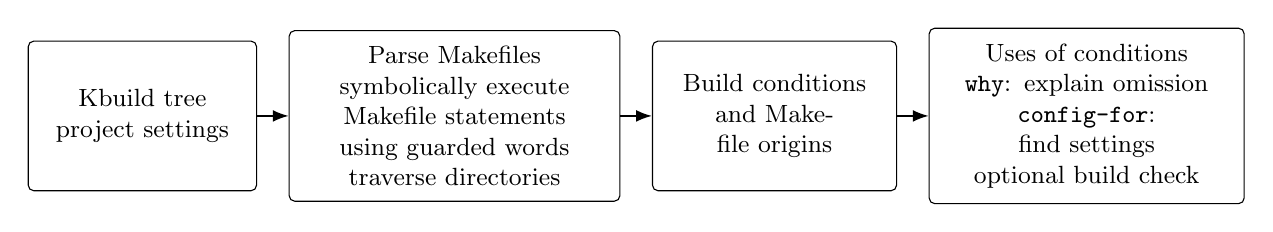
\begin{tikzpicture}[>=Latex,node distance=4mm,
  stage/.style={draw=black,rounded corners=2pt,align=center,inner sep=2mm,minimum height=19mm,font=\small}]
\node[stage,text width=25mm] (input) {Kbuild tree\\project settings};
\node[stage,text width=38mm,right=of input] (analysis) {Parse Makefiles\\symbolically execute\\Makefile statements\\using guarded words\\traverse directories};
\node[stage,text width=27mm,right=of analysis] (map) {Build conditions\\and Makefile origins};
\node[stage,text width=36mm,right=of map] (queries) {Uses of conditions\\\texttt{why}: explain omission\\\texttt{config-for}: find settings\\optional build check};
\draw[->,line width=0.6pt] (input)--(analysis);
\draw[->,line width=0.6pt] (analysis)--(map);
\draw[->,line width=0.6pt] (map)--(queries);
\end{tikzpicture}}
\caption{\tool evaluates Kbuild rules to obtain reusable build conditions and origins.
The rightmost box shows optional downstream queries: \texttt{why} explains a build verdict, while \texttt{config-for} proposes a configuration for selected files; a build can check the proposal.}
\Description{A compact left-to-right flow from a Kbuild tree and project settings through symbolic execution over guarded words to build conditions and Makefile origins, then to optional why and config-for queries with an optional build check.}
\label{fig:overview-pipeline}
\end{figure}

Given a source tree containing the Makefile in Figure~\ref{fig:kbuild-example}, \tool derives the built-in and module conditions in Table~\ref{tab:overview-conditions}.
The Makefile uses option and object names from the Linux \NLinuxVersion \texttt{fs/ext4/Makefile}, with a constructed overwrite and branch to expose the analysis.
Both EXT4 options are tristate, so each can be \texttt{y}, \texttt{m}, or disabled.
In a generated Makefile, disabled \texttt{n} expands to an empty value and contributes to neither \texttt{obj-y} nor \texttt{obj-m}.
Write $E_y$ and $E_m$ for the two enabled values of \texttt{CONFIG\_EXT4\_FS}, and $T_y$ and $T_m$ for those of \texttt{CONFIG\_EXT4\_KUNIT\_TESTS}.
\texttt{CONFIG\_FS\_VERITY} is Boolean, so $V$ means it is \texttt{y} and $\neg V$ means it is disabled.
Kconfig also defines string, integer, and hexadecimal symbols, although this example uses none of them.

% Source names: work/prepared/linux-7.2.8/fs/ext4/Makefile.
% The conditional overwrite and EXTRA branch below are illustrative changes.
\begin{figure}[t]
\centering
\begin{minipage}[t]{0.48\linewidth}
\vspace{0pt}
\begin{lstlisting}[style=kbuild-example]
# Adapted from Linux 7.2.8 fs/ext4/Makefile
obj-$(CONFIG_EXT4_FS) += ext4.o
obj-$(CONFIG_EXT4_KUNIT_TESTS) := ext4-test.o
ifeq ($(CONFIG_FS_VERITY),y)
  EXTRA := verity
else
  EXTRA := crypto
endif
obj-y += $(EXTRA).o
ext4-test-y += inode-test.o
\end{lstlisting}
\captionof{figure}{Input Makefile for the \tool walkthrough, adapted from Linux \NLinuxVersion \texttt{fs/ext4/Makefile}.
The overwrite and \texttt{EXTRA} branch are constructed for this walkthrough and are not verbatim Linux build rules.}
\Description{An adapted Kbuild Makefile with assignments to option-dependent obj variables, a conditional choosing between verity and crypto, an append to obj-y, and an inode-test member of a composite object.}
\label{fig:kbuild-example}
\end{minipage}\hfill
\begin{minipage}[t]{0.48\linewidth}
\vspace{0pt}
\captionof{table}{Local build conditions for Figure~\ref{fig:kbuild-example} before directory guards are applied.
The columns distinguish selection through \texttt{obj-y} and \texttt{obj-m}.}
\label{tab:overview-conditions}
\vspace{6pt}
\centering\small
\begin{tabular}{@{}lll@{}}
\toprule
Target or member & Built-in & Module \\
\midrule
\texttt{ext4.o} & $E_y\land\neg T_y$ & $E_m\land\neg T_m$ \\
\texttt{ext4-test.o} & $T_y$ & $T_m$ \\
\texttt{inode-test.o} & $T_y$ & $T_m$ \\
\texttt{verity.o} & $V$ & --- \\
\texttt{crypto.o} & $\neg V$ & --- \\
\bottomrule
\end{tabular}
\end{minipage}
\end{figure}

\tool expands the first assignment destination to \texttt{obj-y} under $E_y$ and \texttt{obj-m} under $E_m$, adding \texttt{ext4.o} to the corresponding list.
The second assignment replaces \texttt{obj-y} under $T_y$ and \texttt{obj-m} under $T_m$, leaving the other list intact in each case.
Thus \texttt{ext4.o} survives as built-in under $E_y\land\neg T_y$ and as a module under $E_m\land\neg T_m$.
The condition for \texttt{ext4.o} depends on an assignment that does not name it.

Next, \tool evaluates both arms of the conditional and merges \texttt{EXTRA=verity} under $V$ with \texttt{EXTRA=crypto} under $\neg V$.
Expanding \texttt{\$(EXTRA).o} adds \texttt{verity.o} or \texttt{crypto.o} to \texttt{obj-y}, so this assignment has no module route.
\tool records \texttt{inode-test.o} as a member of \texttt{ext4-test.o}.
The member follows its parent's built-in or module selection.

Table~\ref{tab:overview-conditions} describes target-list selection and composite membership within this Makefile.
A selected built-in composite does not necessarily produce a separate object file named after its parent.
For a nested Makefile, \tool then conjoins built-in selections with the guard $B$ for reaching the directory through a built-in route and module selections with the directory reachability guard $D$.
For example, \texttt{ext4.o} has the built-in condition $B\land E_y\land\neg T_y$ and the module condition $D\land E_m\land\neg T_m$.
Either route can select the object, so its overall build condition is $(B\land E_y\land\neg T_y)\lor(D\land E_m\land\neg T_m)$.
\tool also joins conditions with $\lor$ when separate Makefile assignments or directory paths select the same object.
These formulas describe the supported Kbuild analysis, while Kconfig feasibility and physical compilation are checked separately.

These build conditions support the two queries in Figure~\ref{fig:overview-pipeline}.
Given a \texttt{.config}, \tool's \texttt{why} command evaluates an object\textquotesingle s build condition and identifies the first failed part of its condition chain.
For example, if $B$, $E_y$, and $T_y$ hold, \texttt{why} reports that \texttt{ext4.o} is not selected because the later assignment replaced its \texttt{obj-y} entry.
The adapted example does not model Kconfig constraints, so this verdict concerns only its Makefile selection.



Given changed \texttt{.c} or \texttt{.S} files, or a patch, \tool's \texttt{config-for} command maps the touched source files to objects.
\tool combines their build conditions with the relevant Kconfig constraints and seeks a configuration close to a supplied base configuration.
It returns a fragment of option changes and reports files it cannot map or select together.
% Evidence: results/devtasks/config_for.json and config_for_compile.json, commit 82699d1b727b.
For example, a Linux \NLinuxVersion stable fix (``Bluetooth: coredump: Quiesce dump work on unregister'') touches \texttt{net/bluetooth/coredump.c} and \texttt{hci\_core.c}.
Both are members of the composite \texttt{bluetooth.o}, and \texttt{coredump.o} also requires \texttt{CONFIG\_DEV\_COREDUMP}, an option without a prompt that is on only when some driver selects \texttt{WANT\_DEV\_COREDUMP}.
Starting from \texttt{defconfig}, where Bluetooth is off, \texttt{config-for} proposes \texttt{CONFIG\_BT=m} and \texttt{CONFIG\_BT\_HCIVHCI=m}, a driver that selects \texttt{WANT\_DEV\_COREDUMP}, together with the values these imply; the configuration survived \texttt{make olddefconfig}, and both objects compiled.
This Linux task supplies the Kconfig and build checks that the adapted Makefile cannot illustrate.

Applying the fragment through \texttt{make olddefconfig} checks whether the configurator preserves the requested values.
Compiling the selected object checks whether the proposed settings reach a physical build in that task.
A satisfying build condition alone establishes neither result, so \tool reports the proposal and its verification separately.
The next section explains how guarded execution and conditional directory traversal produce the map from object paths to build conditions.

\section{Technique}\label{sec:technique}

This section describes how \tool extracts reusable build conditions from Kbuild Makefiles and uses them to answer developer queries.
We first formalize the analysis setting and state the two core algorithms.
The remaining subsections explain include splicing, guarded assignments, branch merging, directory reachability, physical build semantics, and query evaluation.

\subsection{Setting and Problem Formulation}\label{sec:technique:setting}

Let $M$ denote the set of Kbuild Makefiles across a source repository, and let $c$ denote a configuration that assigns values to configuration options $\mathcal{O}$.
Each option in $\mathcal{O}$ is Boolean ($\texttt{y}$ or unset), tristate ($\texttt{y}$, $\texttt{m}$, or unset), or valued (string, integer, or hexadecimal).
We encode a Boolean or tristate option as one propositional variable per enabled value (e.g., $E_y$ and $E_m$, at most one true), and a Make test that compares a valued option with a literal as an atomic proposition over that option.
For an object path $o$, let $S_M(o, c)$ hold when the build system compiles $o$ under configuration $c$.
\tool computes a propositional formula $\Phi_M(o)$ over option variables such that evaluating $\Phi_M(o)$ under $c$ predicts $S_M(o, c)$.

To compute these formulas without enumerating configurations, \tool represents the value of each Make variable as a mapping from whitespace-separated words to build conditions.
(Variability and software product line literature often refers to configuration formulas guarding code or assets as presence conditions~\cite{liebig2010analysis,thum2014potential,berger2013variability,apel2013feature}.)
Throughout this paper, we consistently use the term \emph{build condition} to denote the propositional formula over configuration options under which a Make variable word, directory route, or compiled object file is selected.
Formally, an execution state $\sigma$ maps each variable name $n$ to a guarded word set $\sigma[n] = \{w \mapsto \phi_w\}$, where $\phi_w$ is a propositional build condition denoting when word $w$ belongs to variable $n$.
We write $\sigma[n](w) = \bot$ when word $w$ is absent from variable $n$.
For two guarded word sets, $\sigma_1[n] \sqcup \sigma_2[n]$ denotes their pointwise disjunction, where the build condition of each word $w$ becomes $\sigma_1[n](w) \lor \sigma_2[n](w)$.

\begin{algorithm}[t]
\caption{Extract guarded Kbuild object conditions}
\label{alg:extract}
\begin{algorithmic}[1]
\Require Source tree $M$, guarded entry files $E$, project settings $\Gamma$
\Ensure Map $\Phi$ from object paths to build conditions and origins
\State $R[m] \gets \bot$ for each file $m \in M$; $Q \gets E$
\State $C \gets \text{empty map}$; $I \gets \emptyset$
\While{$Q$ is nonempty}
  \State remove $(m, \gamma)$ from $Q$
  \State $\delta \gets \gamma \land \neg R[m]$
  \If{$\delta$ is unsatisfiable}
    \State \textbf{continue}
  \EndIf
  \If{$C[m]$ is undefined}
    \State $C[m] \gets \textsc{Exec}(\operatorname{reduce}(\operatorname{splice}(\operatorname{parse}(m))), \sigma_\Gamma, \top)$
  \EndIf
  \State $S \gets \operatorname{restrict}(C[m], \delta)$
  \State $R[m] \gets R[m] \lor \gamma$; add $S$ to $I$
  \For{each selected directory $(d, \eta)$ in $S$}
    \State add $(\operatorname{entry}(d), \eta)$ to $Q$ if its entry file exists
  \EndFor
\EndWhile
\State $\Phi \gets \emptyset$
\For{each restricted instance $S \in I$}
  \For{each target, member, or program object $(o, \phi) \in \operatorname{objects}(S, \Gamma)$}
    \State $\Phi[o] \gets \Phi[o] \lor \phi$ \Comment{initially $\bot$}
  \EndFor
\EndFor
\State $\Phi \gets \operatorname{close}(\Phi, I, \Gamma)$ \Comment{resolve composite members, built-in routes, and rules}
\State \Return $\Phi$
\end{algorithmic}
\end{algorithm}

Algorithm~\ref{alg:extract} presents the end-to-end extraction procedure.
Lines 1--2 initialize the worklist $Q$ with the configured entry files and set the accumulated reachability guard $R[m]$ for every file to false.
Lines 3--17 process reachable Makefiles along incoming directory paths.
For each work item $(m, \gamma)$, line 5 computes the incremental guard $\delta = \gamma \land \neg R[m]$ that has not yet been explored for $m$.
If $\delta$ is unsatisfiable, lines 6--8 discard the item.
Otherwise, lines 9--11 execute the parsed and spliced Makefile under an unrestricted guard when encountering $m$ for the first time, caching the result in $C[m]$.
Line 12 restricts the cached state $C[m]$ to the active guard $\delta$, producing an analyzed instance $S$, and line 13 records $S$ and updates $R[m]$.
Lines 14--16 extract downstream directories selected in $S$ and queue their entry Makefiles under their respective directory guards $\eta$.
After the traversal terminates, lines 18--23 aggregate target words across all recorded instances.
Finally, line 24 computes the transitive closure over composite members, built-in directory reachability constraints, and rule prerequisites before returning the completed map $\Phi$.

\begin{algorithm}[t]
\caption{\textsc{Exec}: execute one statement over guarded words}
\label{alg:exec}
\begin{algorithmic}[1]
\Require Statement $s$, state $\sigma$, ambient guard $g$
\Ensure Updated state $\sigma$
\If{$s$ is an assignment $x\ \mathit{op}\ e$}
  \State $V \gets \{w \mapsto \phi_w\}$ from $\operatorname{expand}(e, \sigma)$, or $\{e \mapsto \top\}$ if $\mathit{op}$ defers $e$ and $e$ contains a reference
  \For{each guarded variable name $(n, \psi_n) \in \operatorname{expand}(x, \sigma)$}
    \State $\psi \gets g \land \psi_n$
    \If{$\mathit{op} \in \{\texttt{=}, \texttt{:=}\}$ or $\sigma[n]$ is undefined}
      \State $\sigma[n] \gets \{w \mapsto \psi \land \phi_w\} \sqcup \{w \mapsto \phi \land \neg\psi : (w \mapsto \phi) \in \sigma[n]\}$
    \Else \Comment{$\mathit{op} = \texttt{+=}$}
      \State $\sigma[n] \gets \sigma[n] \sqcup \{w \mapsto \psi \land \phi_w\}$
    \EndIf
  \EndFor
\ElsIf{$s$ is a conditional with test $t$, then-arm $T$, else-arm $F$}
  \State $\kappa \gets \operatorname{cond}(t, \sigma)$; $\sigma_t \gets \text{copy of } \sigma$; $\sigma_e \gets \text{copy of } \sigma$
  \State $\textsc{Exec}(T, \sigma_t, g \land \kappa)$; $\textsc{Exec}(F, \sigma_e, g \land \neg\kappa)$
  \For{each variable name $n$ assigned in $T$ or $F$}
    \If{$\sigma_t[n](w) = \sigma_e[n](w) = \phi$}
      \State $\sigma[n](w) \gets g \land \phi$ \Comment{fast-path merge for untouched words}
    \Else
      \State $\sigma[n](w) \gets (g \land \kappa \land \sigma_t[n](w)) \lor (g \land \neg\kappa \land \sigma_e[n](w))$
    \EndIf
  \EndFor
\EndIf
\State \Return $\sigma$
\end{algorithmic}
\end{algorithm}

Algorithm~\ref{alg:exec} defines the symbolic execution routine \textsc{Exec} for individual Make statements.
Lines 1--10 handle variable assignments by expanding both the destination variable name and the assigned expression into guarded words.
Lines 11--20 handle conditionals by evaluating the test condition, executing both branches on separate copies of the state, and merging modified variables back into $\sigma$.
We now examine each stage of this analysis in detail.

\subsection{Parsing, Include Splicing, and Dependency Reduction}\label{sec:technique:include}

\tool reads each Makefile and parses its syntax with \texttt{pymake3}.
In Kbuild, an \texttt{include} directive evaluates a referenced file within the environment of the including Makefile, using the repository root as its working directory.
\tool mirrors this behavior through \emph{static include splicing}: it resolves the path of each included file and substitutes the directive with the parsed statements of the target file before running symbolic execution.
Path resolution evaluates standard Kbuild variables such as \texttt{src}, \texttt{obj}, and \texttt{srctree}, as well as constant assignments and string functions such as \texttt{addprefix} and \texttt{addsuffix}.
For example, the Linux AMD GPU driver defines \texttt{FULL\_AMD\_PATH=\$(src)/..} and includes the Makefiles of its sub-drivers through it; the display driver's Makefile in turn builds the paths of its display-library Makefiles with \texttt{addprefix} and \texttt{addsuffix} and includes them.
Without splicing, \NLinuxNoIncludesAllmodconfigLostAmd compiled \texttt{allmodconfig} objects under \path{drivers/gpu/drm/amd/} and \NLinuxNoIncludesAllmodconfigLostNouveau under \path{drivers/gpu/drm/nouveau/} fall outside the extracted set.
When an include path depends on dynamic shell outputs or unresolvable variables, \tool records the unmerged include and continues analysis.

After splicing includes, \tool performs static dependency reduction.
Many statements in Kbuild Makefiles manipulate compiler flags (such as \texttt{ccflags-y} and \texttt{CFLAGS}) that do not affect which object files are selected.
\tool computes the backward dependency cone of all target-affecting variables, composite lists, subdirectories, and build rules.
It then removes statements that do not influence these variables before invoking \textsc{Exec}.
This reduction discards irrelevant flag manipulations, keeping subsequent symbolic execution focused on target selection.

\subsection{Guarded Assignment and Name Expansion}\label{sec:technique:assign}

Kbuild Makefiles construct target lists by appending and assigning to variables whose names and values contain option references.
Algorithm~\ref{alg:exec} evaluates an assignment $x\ \mathit{op}\ e$ by expanding the left-hand name $x$ into a set of guarded variable names $\{(n, \psi_n)\}$ and the right-hand expression $e$ into a set of guarded words $\{(w, \phi_w)\}$.
The effective guard for writing word $w$ into variable $n$ is $\psi = g \land \psi_n \land \phi_w$, where $g$ is the ambient execution guard.

When an assignment appends to a variable ($\mathit{op} = \texttt{+=}$), line 8 joins the new guarded words into $\sigma[n]$ using pointwise disjunction $\sqcup$.
When an assignment overwrites a variable ($\mathit{op} \in \{\texttt{=}, \texttt{:=}\}$), line 6 updates the state conditionally.
The assigned words receive the active guard $\psi \land \phi_w$.
Crucially, any pre-existing word $(w \mapsto \phi)$ in $\sigma[n]$ survives under the narrowed condition $\phi \land \neg\psi$, reflecting that the overwrite replaced the previous definition only in configurations where $\psi$ holds.
A conditional default (\texttt{?=}) leaves existing words untouched and adds each new word under $\psi \land \phi_w \land \neg\bigvee_{w'} \sigma[n](w')$, that is, only where the variable holds no words; Algorithm~\ref{alg:exec} omits this case for brevity.

Consider the following pair of Kbuild assignments:
\begin{lstlisting}[style=kbuild-example]
obj-$(CONFIG_A) += a.o
obj-$(CONFIG_B) := b.o
\end{lstlisting}
Assuming an initially empty state $\sigma[\texttt{obj-y}] = \emptyset$, line 1 expands the destination to \texttt{obj-y} under $A_y = (\texttt{CONFIG\_A=y})$.
Appending \texttt{a.o} yields $\sigma[\texttt{obj-y}] = \{\texttt{a.o} \mapsto A_y\}$.
Line 2 then expands its destination to \texttt{obj-y} under $B_y = (\texttt{CONFIG\_B=y})$.
Because line 2 is an overwrite (\texttt{:=}), \tool assigns \texttt{b.o} under $B_y$ and narrows the existing entry \texttt{a.o} by $\neg B_y$, producing the updated state $\sigma[\texttt{obj-y}] = \{\texttt{a.o} \mapsto A_y \land \neg B_y,\ \texttt{b.o} \mapsto B_y\}$.
The build condition of \texttt{a.o} accurately captures that \texttt{b.o} replaces it whenever $B_y$ holds.

\begin{table}[t]
\centering\footnotesize
\caption{Kbuild Make constructs and \tool's modeled semantics.}
\label{tab:make-scope}
\begin{tabular}{p{28mm}p{48mm}p{48mm}}
\toprule
Construct & Modeled Semantics & Boundary \\
\midrule
\texttt{+=}, \texttt{=}, \texttt{:=}, \texttt{::=} & Guarded words; GNU Make flavor handling (\texttt{::=} as \texttt{:=}); deferred target lists expanded at file end & Word ordering and duplicate occurrences are not preserved. \\
\texttt{?=} & Assigned under the configurations in which the variable holds no words & Differs from GNU Make when a variable is defined but empty. \\
\texttt{ifeq}, \texttt{ifneq}, \texttt{ifdef}, \texttt{ifndef} & Evaluates condition guard, executes both arms on copies, merges modified variables & Tests inherit the limits of variable references below. \\
Variable references & Guarded words plus empty string alternative; substitution references per word & Concatenation collapses when alternatives exceed 64 combinations. \\
Text functions & Handled symbolically for \texttt{filter}, \texttt{patsubst}, \texttt{addprefix}, \texttt{addsuffix}, \texttt{word} & Arbitrary custom recursive functions are unrolled to a fixed depth. \\
\texttt{include} & Recursively spliced when target path resolves statically & Unresolved dynamic include paths contribute no statements. \\
\texttt{\$(eval ...)} & Each guarded expansion of the argument parsed and executed in place under its guard & Text that cannot be parsed contributes no statements. \\
Rules and sub-makes & Targets and prerequisites captured as guarded lists; followed to closure & Recipes other than sub-makes are not executed. \\
\texttt{\$(shell ...)} & Executed as concrete subprocess with timeout; empty in sandbox mode & Output reflects the host environment and installed tools. \\
\bottomrule
\end{tabular}
\end{table}

\tool models GNU Make variable expansion flavors.
For simply expanded assignments (\texttt{:=}), \tool expands the right-hand expression immediately during execution.
For recursively expanded assignments (\texttt{=}) and conditional defaults (\texttt{?=}), \tool stores unexpanded expression text containing variable references and defers evaluation until the end of the Makefile.
This deferred expansion matches Kbuild semantics, because Kbuild reads final target variables only after processing the complete file.
For example, in Linux's \texttt{drivers/xen/Makefile}, the assignment \texttt{dom0-y += \$(xen-pad-y)} precedes the definition of \texttt{xen-pad-y}; deferred evaluation correctly resolves the reference to include \texttt{xen-acpi-pad.o}.
Kbuild Makefiles also generate statements with \texttt{\$(eval)}.
In Linux's \texttt{drivers/platform/x86/intel/Makefile}, for example, \texttt{intel-target-\$(CONFIG\_INTEL\_HID\_EVENT) += hid.o} lists a driver, and the line \texttt{\$(foreach target, \$(basename \$(intel-target-y)), \$(eval \$(call INTEL\_OBJ\_TARGET,\$(target),y)))} expands a two-line \texttt{define} that creates the composite \texttt{intel-hid.o} with member \texttt{hid.o} and appends it to \texttt{obj-y}.
\tool expands the argument of \texttt{\$(eval)} into guarded text alternatives, conjoining the guards of the enclosing \texttt{\$(foreach)} word and \texttt{\$(call)} definition, and executes each alternative as Makefile statements under its guard at the position of the \texttt{\$(eval)}.
Because \texttt{\$(foreach)} visits each word of \texttt{intel-target-y} under that word's own guard, \texttt{intel-hid.o} is selected exactly under \texttt{CONFIG\_INTEL\_HID\_EVENT=y}.
Dependency reduction (\S\ref{sec:technique:include}) executes the evaluated statements as well, so the variables they define and read are kept.
Table~\ref{tab:make-scope} summarizes the supported Make constructs and their operational boundaries.

\subsection{Conditional Execution and Branch Merging}\label{sec:technique:merge}

Kbuild Makefiles make extensive use of conditional directives (\texttt{ifeq}, \texttt{ifneq}, \texttt{ifdef}, and \texttt{ifndef}).
When encountering a conditional statement, Algorithm~\ref{alg:exec} evaluates the test expression $t$ under the current state $\sigma$ to produce a guard formula $\kappa$.
For equality tests, \tool expands both sides into guarded strings and defines $\kappa$ as the disjunction of guards where the two sides coincide.
For example, testing \texttt{ifeq (\$(CONFIG\_FS\_VERITY),y)} produces $\kappa = V$.

Rather than forking the entire execution path into separate analysis branches, \tool creates copies of the state $\sigma_t$ and $\sigma_e$ for the then-arm and else-arm (line 12).
It executes the then-arm $T$ under ambient guard $g \land \kappa$ and the else-arm $F$ under $g \land \neg\kappa$ (line 13).
Lines 14--19 then merge modified variables back into $\sigma$.
For each variable $n$ assigned in either branch, an entry present with guard $\phi_t$ in the then-branch and $\phi_e$ in the else-branch receives the combined guard $(g \land \kappa \land \phi_t) \lor (g \land \neg\kappa \land \phi_e)$.
Conjoining the ambient guard $g$ is safe inside nested conditionals: the enclosing merge re-gates the whole arm with its own branch guard and restores the configurations outside $g$ from the other arm.

To illustrate the contrast between path forking and \tool's state folding, consider sequential conditionals:
\begin{lstlisting}[style=kbuild-example]
ifeq ($(CONFIG_A),y)
  obj-y += a.o
endif
ifeq ($(CONFIG_B),y)
  obj-y += b.o
endif
\end{lstlisting}
A classic path-forking symbolic executor forks at each conditional, maintaining $2^2 = 4$ separate path environments:
$\pi_1(A \land B) \mapsto \{\texttt{a.o}, \texttt{b.o}\}$, $\pi_2(A \land \neg B) \mapsto \{\texttt{a.o}\}$, $\pi_3(\neg A \land B) \mapsto \{\texttt{b.o}\}$, and $\pi_4(\neg A \land \neg B) \mapsto \emptyset$.
For $k$ sequential blocks, path forking produces $O(2^k)$ execution paths.

In contrast, \tool folds branch states at each \texttt{endif} in linear time.
After block 1, \tool holds the single folded state $\sigma[\texttt{obj-y}] = \{\texttt{a.o} \mapsto A\}$.
When evaluating block 2, the then-arm produces $\sigma_t[\texttt{obj-y}] = \{\texttt{a.o} \mapsto A, \texttt{b.o} \mapsto B\}$ under ambient guard $B$, while the else-arm produces $\sigma_e[\texttt{obj-y}] = \{\texttt{a.o} \mapsto A\}$ under $\neg B$.
At the join point, \tool observes that \texttt{a.o} carries the exact same guard $A$ in both arms ($\sigma_t[\texttt{obj-y}](\texttt{a.o}) = \sigma_e[\texttt{obj-y}](\texttt{a.o}) = A$).
Line 16 applies the fast-path merge, setting the guard of \texttt{a.o} directly to $g \land A = A$ (here $g = \top$) rather than creating the redundant disjunction $(B \land A) \lor (\neg B \land A)$.
The final state is $\{\texttt{a.o} \mapsto A,\ \texttt{b.o} \mapsto B\}$, computed in $O(k)$ linear time without path explosion.
The identity $(g \land \kappa \land \phi) \lor (g \land \neg\kappa \land \phi) \equiv g \land \phi$ makes this simplification exact.

\subsection{Conditional Directory Reachability}\label{sec:technique:worklist}

Kbuild orchestrates large source trees hierarchically: a parent Makefile descends into subdirectories listed in target variables and subdirectory lists (\texttt{obj-y}, \texttt{obj-m}, \texttt{subdir-y}, and \texttt{subdir-m}).
Algorithm~\ref{alg:extract} explores this directory structure using a worklist $Q$ starting from top-level entry files $E$.

A naive traversal using a Boolean visited set would fail when the same directory is reachable through multiple independent paths with different configuration guards.
Conversely, re-executing a Makefile on every visit would lead to redundant work.
\tool resolves this trade-off by maintaining an accumulated reachability guard $R[m]$ for each Makefile $m$.
When a work item $(m, \gamma)$ is dequeued, line 5 computes the uncovered guard $\delta = \gamma \land \neg R[m]$.
If Z3 determines that $\delta$ is unsatisfiable, the visit is redundant and skipped.
Otherwise, lines 9--11 obtain the cached baseline execution state $C[m]$ and line 12 restricts it by conjoining all guards with $\delta$.
Line 13 updates $R[m] \gets R[m] \lor \gamma$.
Lines 14--16 then extract directory targets and append child Makefiles to $Q$ alongside their reachability guards $\eta$.

Consider a top-level Makefile that reaches a subdirectory through two independent option routes:
\begin{lstlisting}[style=kbuild-example]
obj-$(CONFIG_NET) += drivers/net/
obj-$(CONFIG_PCI) += drivers/net/
\end{lstlisting}
When processing the first entry under guard $N$ (for \texttt{CONFIG\_NET=y}), \tool executes \path{drivers/net/Makefile} once under $\top$, caches its execution state $C[\texttt{net}]$, restricts it to $N$, and records $R[\texttt{net}] = N$.
When the second entry arrives under guard $P$ (for \texttt{CONFIG\_PCI=y}), \tool computes $\delta = P \land \neg N$.
If Z3 determines that $\delta$ is satisfiable, \tool restricts the cached state $C[\texttt{net}]$ by $\delta$, updates $R[\texttt{net}] = N \lor P$, and queues newly reachable subdirectories.
If $P$ already implies $N$, $\delta$ is unsatisfiable and \tool skips the visit entirely.
Because the source repository contains a finite number of Makefiles and option domains are finite, $R[m]$ can strictly weaken only finitely many times, guaranteeing termination.

\subsection{Object Extraction and Kbuild Build Semantics}\label{sec:technique:build}

After the directory worklist terminates, \tool extracts physical object paths from the recorded instances $I$.
Target extraction inspects standard Kbuild target families (\texttt{obj-}, \texttt{lib-}, \texttt{extra-}, and \texttt{always-}) as well as project-specific families (such as \texttt{pbl-} in Barebox and \texttt{bootblock-} in coreboot).
\tool models four core build semantics from Kbuild's \texttt{scripts/Makefile.build}:

\paragraph{Composite Object Resolution.}
When a selected target $t$ represents a composite object, Kbuild compiles its constituent members rather than a single source file of the same name.
\tool inspects composite definitions in variables such as \texttt{$t$-y}, \texttt{$t$-objs}, \texttt{$t$-lib}, and \texttt{$t$-m}.
It assigns each member object the conjunction of its own guard and the container object's guard.
In Linux \NLinuxVersion, composite members account for \NLinuxMembers of the \NLinuxObjects analyzed object paths.

\paragraph{Built-in Containers and Objects.}
When a composite target is selected for a built-in build (\texttt{obj-y}), Kbuild links its member objects directly into the directory's archive (\texttt{built-in.a}) and produces no standalone object file for the container name.
Only module composites (\texttt{obj-m}) generate container object files on disk.
\tool therefore suppresses built-in composite container paths from the final object map while preserving their member objects.

\paragraph{Built-in Directory Reachability Routes.}
Kbuild sets an internal flag \texttt{need-builtin} during recursive builds: a directory builds its \texttt{built-in.a} archive and its \texttt{obj-y} targets only if the parent directory was entered through an \texttt{obj-y} reference.
If a directory is reached solely through an \texttt{obj-m} or \texttt{subdir-y} reference, Kbuild builds its modules and auxiliary targets but skips its \texttt{obj-y} objects.
\tool computes the built-in reachability guard $B_m$ for every Makefile $m$ as a fixpoint over \texttt{obj-y} directory edges and conjoins $B_m$ with every built-in object guard.

\paragraph{Rule Prerequisites and Sub-makes.}
Certain kernel objects do not appear in target lists and are built only when invoked as prerequisites of explicit or pattern rules.
For example, vDSO objects and boot images are compiled through architecture-specific rules in \texttt{arch/x86/entry/vdso/} and \texttt{arch/x86/boot/Makefile}: the vDSO image object is compiled from a C file that a pattern rule generates from a shared object, which an explicit rule links from the vDSO objects.
\tool records explicit rules, pattern rules, and sub-make invocations of the form \texttt{\$(MAKE) \$(build)=\textit{dir} \textit{goal}} as guarded structures.
Line 24 of Algorithm~\ref{alg:extract} computes a prerequisite closure starting from all selected objects, the non-object targets of \texttt{always-} and \texttt{extra-} lists, and configured goals, pulling in rule prerequisites under the conjunction of their triggering guards.
As in GNU Make, a pattern rule applies only if each of its prerequisites exists or can be made.
For instance, \texttt{kernel/trace/Makefile} adds \texttt{simple\_ring\_buffer.o.checked} to \texttt{always-\$(CONFIG\_SIMPLE\_RING\_BUFFER)}, and the pattern rule for \texttt{\%.o.checked} needs \texttt{undefsyms\_base.o}, which no list names.

\subsection{Applications: Developer Queries and Analysis Cache}\label{sec:technique:queries}

The resulting map $\Phi$ stores the exact build conditions and origin Makefiles for all discovered objects.
\tool uses this map to answer developer queries about the project build without re-analyzing the source tree. 

\paragraph{Explaining Omissions (\texttt{why}).}
Given a configuration file \texttt{.config} and a target object path $o$, \tool evaluates $\Phi(o)$ under the supplied configuration.
If the condition evaluates to false, \tool traverses the chain of conditions that produced $\Phi(o)$---including directory reachability, assignment guards, and composite membership---and identifies the first unsatisfied guard term.
This pinpoints whether the object was omitted due to an unset top-level option, a directory bypass, or an overwrite in a specific Makefile.

\paragraph{Enabling Changed Files (\texttt{config-for}).}
Given a set of modified source files or a patch, \tool maps each source file to its corresponding object path $o$ and retrieves build condition $\Phi(o)$.
To ensure that the requested options can be enabled without violating kernel dependencies, \tool extracts the Kconfig dependency cone for all options appearing in $\Phi(o)$: the options reachable through \texttt{depends on}, prompt and default conditions, and choices, built with \texttt{kconfiglib} and extended for Kconfig syntax newer than that library.
Its Kconfig encoding $K$ bounds each option from above by its dependencies and from below by its \texttt{select}s, and allows it to be on only through a \texttt{select}, an \texttt{imply}, a visible prompt, or an active default; because it does not decide which default applies, $K$ over-approximates Kconfig.
\tool conjoins the build conditions with $K$ and queries Z3 for a satisfying assignment that minimizes changes relative to a base \texttt{.config}.
An object whose condition is unsatisfiable together with $K$, or that conflicts with another touched object, is reported with the reason.
With verification, \tool applies the fragment with \texttt{make olddefconfig}, checks that every requested option survives, and checks that it predicts every touched object under the result.

\paragraph{Finding Blind Spots (\texttt{blindspots}).}
Given a set of configurations, \tool evaluates every build condition under each of them and reports the objects that none of them builds, grouped by the \texttt{MAINTAINERS} entry that owns the source file and labeled with a likely reason, such as an option of another architecture or an option that none of the configurations enables.

\paragraph{Analysis Cache and Invalidation.}
\tool persists each object's kind, origins, and build condition, together with the reachability conditions of analyzed Makefiles, in a per-tree cache: a JSON metadata file plus the conditions as SMT-LIB terms with shared subterms.
Subsequent invocations of \texttt{why} and \texttt{config-for} load this cache and parse conditions lazily, one object at a time.
The cache records the path, modification time, and size of every Makefile, included fragment, and settings file the analysis read, plus a content hash of the analyzer itself.
If any of these changes, \tool discards the cache and reruns the whole-tree analysis; incremental re-analysis is future work.

\section{Evaluation}
\label{sec:evaluation}

We evaluate whether \tool's conditions predict the objects that real builds produce, how it scales, whether its conditions support developer tasks, and how it compares with \kmax and with itself when design elements are removed.
We ask four research questions:
\begin{itemize}
\tightlist
\item \textbf{RQ1 (Build Agreement):} When the conditions are evaluated under a configuration, how many predicted objects are compiled, and how many compiled objects are predicted? (\S\ref{sec:eval:agreement})
\item \textbf{RQ2 (Scalability and State Folding):} How do \tool's time and memory grow with the number of conditional assignments, compared with a path-forking executor and with \kmax, and what does a whole tree cost? (\S\ref{sec:eval:scaling})
\item \textbf{RQ3 (Developer Diagnostics and Automated Configuration):} Do the conditions explain why an object is or is not built, produce configurations that compile the files a real patch touches, and find code that standard configurations never build? (\S\ref{sec:eval:developer})
\item \textbf{RQ4 (Comparative Analysis and Ablations):} How do \kmax's conditions compare with \tool's against the same builds, and how much does each design element contribute? (\S\ref{sec:eval:comparative})
\end{itemize}

\subsection{Experimental Setup and Provenance}
\label{sec:eval:setup}
The subjects are the latest releases of five Kbuild-based systems (Table~\ref{tab:subjects}): Linux \NLinuxVersion, BusyBox \NBusyboxVersion, Barebox \NBareboxVersion, Das U-Boot \NUbootVersion, and coreboot \NCorebootVersion.
Linux and BusyBox are the two systems in \kmax's evaluation~\cite{gazzillo2017kmax}; Barebox, U-Boot, and coreboot are bootloader and firmware projects whose Kbuild dialects add families for stages or pre-bootloader code.
Each is an unmodified release tarball, checked against the published SHA-256 where the project publishes one.
Linux has four configurations: i386 \texttt{tinyconfig}, x86-64 \texttt{defconfig}, the configuration of the Debian kernel package, and x86-64 \texttt{allmodconfig}; the others have one each.
Each subject's settings copy the directory lists and goals of its top-level Makefiles, with each entry annotated with the lines it comes from; for Linux they name seven directories, three of them guarded, one goal, and the definitions of \texttt{SRCARCH} and \texttt{BITS}.

We built every configuration from scratch with \texttt{make -k}, from \NLinuxTinyconfigBuildMinutes minutes for \texttt{tinyconfig} to \NLinuxAllmodconfigBuildMinutes for \texttt{allmodconfig}, and took as the inventory $B_c$ every \texttt{.o} file in the build tree except the \texttt{*.mod.o} files that \texttt{modpost} generates.
The builds deviate from stock only where the current toolchain or a missing external input requires it: the Debian configuration has its trusted-key lists emptied, \texttt{allmodconfig} has \texttt{-Werror} disabled so that new compiler warnings do not abort files, coreboot builds without a payload, and U-Boot's final image step fails after all objects have compiled.
BusyBox's \texttt{networking/tc.c} no longer compiles against current kernel headers; objects that \texttt{make} attempted and failed to compile are reported separately from false positives.

\begin{table}[t]
\centering\footnotesize
\caption{Subjects, configurations, and the number of \texttt{.o} files in each fresh build.}
\label{tab:subjects}
\begin{tabular}{lllr}
\toprule
Subject & Version & Configuration & Objects built \\
\midrule
\tablebody{subjects}
\bottomrule
\end{tabular}
\end{table}

\emph{Metrics.} \tool emits an extracted object-path set $U$ and a condition for each path.
For a configuration $c$, evaluating the conditions yields a predicted set $P_c\subseteq U$.
We define $TP=|P_c\cap B_c|$, $FP=|P_c\setminus B_c|$, $FN_U=|(B_c\cap U)\setminus P_c|$, and $O=|B_c\setminus U|$, and report precision $TP/(TP+FP)$ and overlap $TP/|B_c|$.
Overlap charges \tool for every compiled object it does not extract, including host tools under \texttt{scripts/} and \texttt{tools/}, which the analyzed Makefiles do not select; $FN_U$ separately counts extracted objects whose condition is false although the object was compiled.
To evaluate a condition, the evaluator substitutes the value of every option in the \texttt{.config}, treating an option that is absent or ``is not set'' as unset.

\emph{Setup.} All runs used an Intel Core i7-7700 with eight logical CPUs and 31\,GiB of RAM under Debian Linux, with Python 3.14.7, Z3 4.13.3, GNU Make 4.4.1, and GCC 16.2.0.
The Linux analysis uses the tristate domain.
Whole-tree times are the median of three runs on an otherwise idle machine.
One script regenerates every result, and every number in this section is generated from its output.

\subsection{RQ1: Build Agreement}
\label{sec:eval:agreement}
On all four Linux configurations, every object that \tool predicts is compiled, and every compiled object that \tool extracts is predicted (Table~\ref{tab:linux-physical}): there is no false positive and no in-set miss, from \NLinuxTinyconfigPred predicted objects for \texttt{tinyconfig} to \NLinuxAllmodconfigPred for \texttt{allmodconfig}.
The predictions include the boot image, real-mode, vDSO, and EFI-stub objects, composite members of modules, and the link artifacts.
Overlap is \NLinuxTinyconfigOverlap--\NLinuxAllmodconfigOverlap\%.
Every compiled object outside $U$ is a host tool under \texttt{scripts/} or \texttt{tools/}, which the analyzed Makefiles do not select, so without host tools overlap is \NLinuxMinOverlapnohost\% on all four configurations.
The predictions include objects that Makefiles create through \texttt{\$(eval \$(call \ldots))}, such as the Intel and Lenovo platform drivers, and \texttt{kernel/trace/undefsyms\_base.o}, which only a pattern rule for an \texttt{always-y} target needs.
The last column shows that composite members are essential: counting only the words of target lists, \tool covers \NLinuxDebianTargetsoverlap--\NLinuxTinyconfigTargetsoverlap\% of each inventory.

\begin{table}[t]
\centering\footnotesize
\caption{Predicted versus compiled Linux \NLinuxVersion objects. $O$ counts compiled objects outside $U$, with host tools in parentheses. ``Targets'' is the overlap when composite members are not resolved.}
\label{tab:linux-physical}
\setlength{\tabcolsep}{3.5pt}
\begin{tabular}{lrrrrrrrrr}
\toprule
Configuration & Built & Pred. & TP & FP & $FN_U$ & $O$ (host) & Prec. & Overlap & Targets \\
\midrule
\tablebody{linux_agreement}
\bottomrule
\end{tabular}
\end{table}

\begin{table}[t]
\centering\footnotesize
\caption{Predicted versus compiled objects for the other subjects. ``Failed'' counts predicted objects that \texttt{make} attempted but could not compile; they are not counted as false positives.}
\label{tab:firmware-physical}
\setlength{\tabcolsep}{3.5pt}
\begin{tabular}{lrrrrrrrrr}
\toprule
Subject & Built & Pred. & TP & FP & Failed & $FN_U$ & $O$ (host) & Prec. & Overlap \\
\midrule
\tablebody{other_agreement}
\bottomrule
\end{tabular}
\end{table}

The other dialects agree as closely (Table~\ref{tab:firmware-physical}): no subject has a false positive or an in-set miss.
The one BusyBox prediction that is not compiled is \texttt{networking/tc.o}, whose compilation fails.
Without host tools, overlap is \NBusyboxDefconfigOverlapnohost\% for BusyBox, \NBareboxSandboxDefconfigOverlapnohost\% for Barebox, \NUbootSandboxDefconfigOverlapnohost\% for U-Boot, and \NCorebootQemuIFFZfxOverlapnohost\% for coreboot.
The rest are BusyBox's \texttt{built-in.o} archives, which its older Kbuild writes as \texttt{.o} files; Barebox's link intermediates and generated blobs, such as its default environment; U-Boot's EFI example applications, which dedicated rules build; and coreboot's mainboard objects, which its top-level Makefile adds through variables that our entry settings do not copy, together with objects built from the generated devicetree and as relocatable modules.

\subsection{RQ2: Scalability and State Folding vs. Path Forking}
\label{sec:eval:scaling}
\emph{Controlled growth.} To isolate the effect of the representation, we generated Makefiles with $k$ independent options in four families: $k$ computed-name appends (\texttt{obj-\$(CONFIG\_A$_i$) += a$_i$.o}); $k$ \texttt{ifeq} blocks that each append to \texttt{obj-y}; $k$ \texttt{ifeq}/\texttt{else} blocks that set a variable used in an object name (\emph{value}); and $k$ \texttt{ifeq} blocks that append to a helper list later appended to \texttt{obj-y} (\emph{indirect}).
For $k$ from 1 to \NBenchMaxk we ran \tool, the forking executor that \tool's per-word representation replaced (the same code base before that change, which forks at each conditional and merges identical paths), and \kmax in both of its output modes, with a limit of \NBenchTimeout\,s per run.

Table~\ref{tab:scaling-bench} shows that \tool's cost does not grow with $k$: all \NBenchKfoldRuns runs take \NBenchKfoldMinSeconds--\NBenchKfoldMaxSeconds\,s, most of it interpreter start-up, and at most \NBenchKfoldMaxRss\,MB, and every run reports exactly the expected objects.
The forking executor's cost depends on how many distinct values the conditionals create.
On \emph{append}, each computed-name assignment forks on one option only, and on \emph{ifeq} it merges the arms into $k+1$ states, yet its time still grows to \NBenchIfeqSFSeconds\,s at $k=64$ and exceeds the limit at $k=128$.
When each conditional sets a value used in a name or extends a helper list, the states multiply: \NBenchValueOTStates states at $k=12$ for \emph{value}, and \NBenchIndirectOSStates states and \NBenchIndirectOSSeconds\,s at $k=16$ for \emph{indirect}; the next sizes time out.
\kmax stays below \NBenchKmaxMaxSeconds\,s in its text output mode and below \NBenchKmaxSmtMaxSeconds\,s in the SMT mode that \texttt{kmaxall} uses, so this benchmark separates per-word guards from path forking rather than \tool from \kmax.
On \emph{value}, both \kmax modes report $k$ objects that no build can produce, such as \texttt{c0\_\$(V0).o}, besides the $2k$ correct ones.

\begin{table}[t]
\centering\footnotesize
\caption{Controlled growth on generated Makefiles with $k$ independent options: states and seconds of the forking executor per family, and the slowest \tool and \kmax (text mode) run over all four families. Times include about 0.5\,s of start-up. ``t/o'' marks the \NBenchTimeout\,s limit and ``--'' a run skipped after a smaller $k$ timed out.}
\label{tab:scaling-bench}
\begin{tabular}{rrrrrr}
\toprule
& \multicolumn{3}{c}{Forking: states / time (s)} & \tool & \kmax \\
\cmidrule(lr){2-4}
$k$ & \emph{ifeq} & \emph{value} & \emph{indirect} & time (s) & time (s) \\
\midrule
\tablebody{scaling}
\bottomrule
\end{tabular}
\end{table}

\emph{Whole trees.} Table~\ref{tab:corpus-timing} gives \tool's cost on the five subjects.
For Linux, it analyzes \NLinuxInstances Makefile instances and extracts \NLinuxObjects object paths (\NLinuxTargets target words and \NLinuxMembers composite members, plus programs and rule prerequisites) in \NLinuxSeconds\,s with \NLinuxRss\,MB and \NLinuxZTchecks Z3 checks; the rule closure and built-in routes are included.
The other subjects take \NBusyboxSeconds--\NCorebootSeconds\,s.
The analysis runs once per tree revision; the developer commands of RQ3 reuse its cached result.
On the same Linux tree, \kmax takes \NLinuxKmaxSeconds\,s and \NLinuxKmaxRssGb\,GB (\S\ref{sec:eval:comparative}).

\begin{table}[t]
\centering\footnotesize
\caption{Whole-tree analysis: median time of three runs and peak resident memory. Object paths include composite members, programs, and rule prerequisites.}
\label{tab:corpus-timing}
\begin{tabular}{lrrrr}
\toprule
Subject & Makefile instances & Object paths & Time (s) & Memory (MB) \\
\midrule
\tablebody{timing}
\bottomrule
\end{tabular}
\end{table}

\subsection{RQ3: Developer Diagnostics and Automated Configuration}
\label{sec:eval:developer}
We ran the three commands of \S\ref{sec:technique:queries} on Linux, using the cached whole-tree analysis.

\emph{Explaining a build (\texttt{why}).} For each of the four built configurations, we drew a seeded random sample of \NWhyPerSide extracted objects that the build produced and \NWhyPerSide that it did not.
For all \NWhyCases objects, the verdict of \texttt{why} matches the build.
For an object that is not built, \texttt{why} names the first part of the condition chain that fails: a directory route in \NWhyFailDirectoryRoute cases, the target-list line in \NWhyFailTargetListLine, and composite membership in \NWhyFailCompositeMembership.
A directory route explains, for instance, the objects under \texttt{drivers/net/wireless/} under \texttt{tinyconfig}, where the build never enters that directory whatever the objects' own lines say.

\emph{Configurations for real patches (\texttt{config-for}).} We used every commit of the Linux 7.2.7-to-7.2.8 stable update that touches a \texttt{.c} or \texttt{.S} file, \NConfigforCommits commits, and ran \texttt{config-for} on each as a patch against \texttt{defconfig}, with verification: the fragment is applied with \texttt{make olddefconfig} and every requested option is checked in the result.
For \NConfigforSelectable commits, \texttt{config-for} produces a verified configuration under which \tool predicts every touched object.
In \NConfigforUnmapped commits no touched file is an object of the x86 tree (for example, selftests and other architectures).
In the remaining \NConfigforExcluded commits, \texttt{config-for} reports a touched object as impossible under Kconfig and Kbuild together; each of these objects needs an option of another architecture, such as \texttt{ARCH\_K3} on arm64 or \texttt{SPARC}.
In every verified configuration, each option that the fragment sets survives \texttt{olddefconfig}.
The median query takes \NConfigforMedianSeconds\,s including verification.
From the \NConfigforSelectable selectable commits we drew \NCompileSampled at random, applied each verified configuration to a copy of the \texttt{defconfig} build tree, and compiled the touched objects: they compiled for \NCompileOk of the \NCompileSampled commits.
The Kconfig model used by \texttt{config-for} is checked separately on \texttt{tinyconfig}, \texttt{defconfig}, Debian, \texttt{allmodconfig}, and \texttt{allyesconfig}: the values that \texttt{kconfiglib} computes agree with those that \texttt{scripts/kconfig} wrote for all \NKconfigDefined options except \NKconfigMismatches under \texttt{allmodconfig}, and each of the five configurations satisfies $K$, so $K$ does not exclude any of them.

\emph{Blind spots.} We asked which extracted objects none of x86-64 \texttt{allmodconfig}, \texttt{allyesconfig}, and \texttt{defconfig} builds.
\tool finds \NBlindBlindSpots of \NBlindObjectsConsidered objects, owned by \NBlindEntriesWithBlindSpots \texttt{MAINTAINERS} entries.
Of these, \NBlindArch need an option of another architecture, such as \texttt{CONFIG\_S390}; \NBlindNotenabled need an option that none of the three configurations enables, and \texttt{blindspots} names it; the remaining \NBlindNopivot have no single such option, among them the containers of built-in composites, which Kbuild never writes as files.
The query shows maintainers which code the usual test configurations never compile.

\subsection{RQ4: Comparative Analysis and Ablations}
\label{sec:eval:comparative}
\emph{\kmax.} We ran \kmax v4.10 the way it analyzes a whole tree: \texttt{kmaxall} in tristate mode from Linux's root \texttt{Kbuild} with \texttt{SRCARCH=x86}, plus \texttt{lib/}, under \texttt{python3 -O}.
As distributed, \texttt{kmaxall} aborts the whole run with a Python~3 \texttt{TypeError} when any directory fails, so we ran a copy with that one error-reporting call fixed.
\kmax took \NLinuxKmaxSeconds\,s and \NLinuxKmaxRssGb\,GB of memory; \texttt{fs/hostfs/} failed with an internal \texttt{KeyError}.
It reports \NLinuxKmaxObjects object paths, \NLinuxKmaxUnexpanded of them with unexpanded references such as \texttt{arch/x86/kernel/apic/probe\_\$(BITS).o}.
Its output gives each object a condition relative to its own Makefile and records each subdirectory's condition separately; we evaluated both the local conditions and the conditions conjoined with every ancestor directory's.

Table~\ref{tab:kmax} compares the two tools on the same four builds.
\kmax's local conditions predict too many objects on small configurations: on \texttt{tinyconfig}, its precision is \NLinuxKmaxTinyconfigLocalPrec\%, with many false positives in directories that the build never enters, such as \texttt{drivers/acpi/}.
Conjoining the directory conditions raises precision but lowers overlap.
In both variants, \kmax misses between \NLinuxKmaxTinyconfigLocalFn and \NLinuxKmaxAllmodconfigWithDirsFn compiled objects that it extracts.
On the three x86-64 configurations, most of them are composite members in \tool's analysis (\NLinuxKmaxAllmodconfigLocalFnMembers of \NLinuxKmaxAllmodconfigLocalFn under \texttt{allmodconfig} with local conditions): \kmax gives a composite's members the condition that the container's option is \texttt{y}, so members of a composite built as a module are never predicted.
On BusyBox, which has no composites, the tools agree: both predict \NBusyboxKmaxDefconfigLocalTp compiled objects with no in-set miss; \kmax takes \NBusyboxKmaxSeconds\,s and \tool \NBusyboxSeconds\,s.

\begin{table}[t]
\centering\footnotesize
\caption{\kmax and \tool against the same Linux builds: precision / overlap (\%) and compiled extracted objects that are not predicted ($FN_U$). ``Local'' uses \kmax's per-Makefile conditions; ``with dirs'' conjoins the conditions it records for ancestor directories.}
\label{tab:kmax}
\setlength{\tabcolsep}{4pt}
\begin{tabular}{lrrrrrr}
\toprule
& \multicolumn{2}{c}{\tool} & \multicolumn{2}{c}{\kmax local} & \multicolumn{2}{c}{\kmax with dirs} \\
\cmidrule(lr){2-3}\cmidrule(lr){4-5}\cmidrule(lr){6-7}
Configuration & P / O & $FN_U$ & P / O & $FN_U$ & P / O & $FN_U$ \\
\midrule
\texttt{tinyconfig} & \NLinuxTinyconfigPrec\,/\,\NLinuxTinyconfigOverlap & \NLinuxTinyconfigFn & \NLinuxKmaxTinyconfigLocalPrec\,/\,\NLinuxKmaxTinyconfigLocalOverlap & \NLinuxKmaxTinyconfigLocalFn & \NLinuxKmaxTinyconfigWithDirsPrec\,/\,\NLinuxKmaxTinyconfigWithDirsOverlap & \NLinuxKmaxTinyconfigWithDirsFn \\
\texttt{defconfig} & \NLinuxDefconfigPrec\,/\,\NLinuxDefconfigOverlap & \NLinuxDefconfigFn & \NLinuxKmaxDefconfigLocalPrec\,/\,\NLinuxKmaxDefconfigLocalOverlap & \NLinuxKmaxDefconfigLocalFn & \NLinuxKmaxDefconfigWithDirsPrec\,/\,\NLinuxKmaxDefconfigWithDirsOverlap & \NLinuxKmaxDefconfigWithDirsFn \\
Debian & \NLinuxDebianPrec\,/\,\NLinuxDebianOverlap & \NLinuxDebianFn & \NLinuxKmaxDebianLocalPrec\,/\,\NLinuxKmaxDebianLocalOverlap & \NLinuxKmaxDebianLocalFn & \NLinuxKmaxDebianWithDirsPrec\,/\,\NLinuxKmaxDebianWithDirsOverlap & \NLinuxKmaxDebianWithDirsFn \\
\texttt{allmodconfig} & \NLinuxAllmodconfigPrec\,/\,\NLinuxAllmodconfigOverlap & \NLinuxAllmodconfigFn & \NLinuxKmaxAllmodconfigLocalPrec\,/\,\NLinuxKmaxAllmodconfigLocalOverlap & \NLinuxKmaxAllmodconfigLocalFn & \NLinuxKmaxAllmodconfigWithDirsPrec\,/\,\NLinuxKmaxAllmodconfigWithDirsOverlap & \NLinuxKmaxAllmodconfigWithDirsFn \\
\bottomrule
\end{tabular}
\end{table}

\emph{Ablation.} We removed one design element at a time and repeated the comparison with the builds (Table~\ref{tab:ablation}); composite members are covered by the last column of Table~\ref{tab:linux-physical}.
Without include splicing, \tool loses \NLinuxNoIncludesLostObjects Linux objects, mostly in the AMD and Nouveau GPU drivers, whose Makefiles list their objects in included files, and overlap drops to \NLinuxNoIncludesDebianOverlap\% on Debian.
Without the rule closure, \tool loses \NLinuxNoRulesLostObjects objects, the boot image, real-mode, and vDSO objects among them, so overlap drops most on \texttt{tinyconfig}, where they are a large share of a small kernel, and objects that are still extracted but reached only through a rule are missed ($FN_U$).
Without the built-in semantics of \S\ref{sec:technique:build}, overlap is unchanged but built-in composite containers and the built-in objects of directories reached only through \texttt{obj-m} are predicted but never written, adding up to \NLinuxNoLinkSemanticsDefconfigFp false positives.
On the other subjects, only the built-in semantics matter: without them, Barebox gains \NBareboxNoLinkSemanticsSandboxDefconfigFp and U-Boot \NUbootNoLinkSemanticsSandboxDefconfigFp false positives.

\begin{table}[t]
\centering\footnotesize
\caption{Ablation on Linux: overlap (\%), in-set misses, and false positives with one design element removed.}
\label{tab:ablation}
\setlength{\tabcolsep}{4pt}
\begin{tabular}{lrrrrr}
\toprule
& Full \tool & No includes & \multicolumn{2}{c}{No rule closure} & No built-in sem. \\
\cmidrule(lr){2-2}\cmidrule(lr){3-3}\cmidrule(lr){4-5}\cmidrule(lr){6-6}
Configuration & Overlap & Overlap & Overlap & $FN_U$ & $FP$ \\
\midrule
\texttt{tinyconfig} & \NLinuxTinyconfigOverlap & \NLinuxNoIncludesTinyconfigOverlap & \NLinuxNoRulesTinyconfigOverlap & \NLinuxNoRulesTinyconfigFn & \NLinuxNoLinkSemanticsTinyconfigFp \\
\texttt{defconfig} & \NLinuxDefconfigOverlap & \NLinuxNoIncludesDefconfigOverlap & \NLinuxNoRulesDefconfigOverlap & \NLinuxNoRulesDefconfigFn & \NLinuxNoLinkSemanticsDefconfigFp \\
Debian & \NLinuxDebianOverlap & \NLinuxNoIncludesDebianOverlap & \NLinuxNoRulesDebianOverlap & \NLinuxNoRulesDebianFn & \NLinuxNoLinkSemanticsDebianFp \\
\texttt{allmodconfig} & \NLinuxAllmodconfigOverlap & \NLinuxNoIncludesAllmodconfigOverlap & \NLinuxNoRulesAllmodconfigOverlap & \NLinuxNoRulesAllmodconfigFn & \NLinuxNoLinkSemanticsAllmodconfigFp \\
\bottomrule
\end{tabular}
\end{table}

\subsection{Threats to Validity}
\label{sec:eval:threats}
\emph{Construct validity.} Precision and overlap compare path names; neither measures whether a source file builds under an arbitrary configuration.
Inventories contain objects that are not ordinary compilation units, such as host tools, BusyBox's \texttt{built-in.o} archives, and generated blobs; the tables list them separately rather than removing them.

\emph{Internal validity.} We developed several of \tool's semantics, including include splicing, the built-in semantics, and the rule closure, while examining discrepancies on Linux builds, so agreement partly reflects fitting to them.
Each addition implements a documented behavior of GNU Make or of Kbuild's \texttt{Makefile.build} and has a regression test on a small Makefile.
Most of them were developed on Linux v6.6; running on \NLinuxVersion exposed two defects in the rule closure, and the objects missed in a first run led us to add \texttt{\$(eval)} and to follow the rules of \texttt{always-y} targets; all of these changes were made before the runs reported here.
Likewise, an earlier \texttt{config-for} run on the same stable patches exposed three options that did not survive \texttt{olddefconfig}; we then made $K$ account for prompt visibility, defaults, and tristate comparisons, and checked the change against the five real configurations rather than against the patches.
The \texttt{why} samples and \texttt{config-for} patches are drawn independently of \tool.
The entry settings copy directory lists and goals from top-level Makefiles by hand, and a copying error would change the traversal.

\emph{External validity.} Linux has four configurations, all x86, and each other system one.
The \texttt{config-for} patches come from one stable update, whose fixes may touch fewer optional drivers than new development does.
The results describe this implementation on these subjects; they do not show that \tool handles every Kbuild dialect or configuration.

\section{Discussion and Limitations}\label{sec:discussion}

\subsection{What Build Conditions Support}\label{sec:discussion:support}

The primary utility of \tool's build conditions is providing transparent, queryable explanations of build-system behavior.
When an object is unexpectedly omitted from a build, maintainers can inspect its build condition to trace the exact chain of configuration requirements, directory reachability guards, and assignment overwrites responsible for the omission.
Furthermore, \tool enables proactive configuration synthesis by translating build conditions into SMT constraints, allowing developers to generate configuration deltas for newly modified files without manual trial and error.

Maintainers should note that a Kbuild-local build condition $\Phi(o)$ denotes the formula under which Makefiles select object $o$.
It does not guarantee that $\Phi(o)$ is satisfiable under global Kconfig rules.
For this reason, \tool combines build conditions with Kconfig dependency cones during \texttt{config-for} queries and verifies synthesized configurations through \texttt{make olddefconfig}; in our evaluation, we also compiled the touched objects of a sample of them.

\subsection{Construct Boundaries and Limitations}\label{sec:discussion:limitations}

\tool models standard Kbuild semantics but faces natural boundaries when encountering unconstrained dynamic Make features:
\begin{itemize}
\tightlist
\item \textbf{Generated and Recipe-Built Objects:} Objects that only a recipe or a generator produces, such as Barebox's embedded default-environment blobs, appear in no list or rule that \tool follows. Evaluated text that cannot be parsed (\texttt{\$(eval)}) contributes no statements.
\item \textbf{Host-Dependent Shell Execution:} Kbuild Makefiles occasionally invoke host utilities via \texttt{\$(shell ...)} to detect compiler capabilities (e.g., \texttt{as-instr} or \texttt{cc-option}). \tool evaluates shell calls concretely in the ambient host environment, which means analysis outcomes may reflect host toolchain capabilities.
\item \textbf{Top-Level Build Orchestration:} \tool does not execute top-level Makefiles; project settings copy their entry directories and goals. Objects that a top-level Makefile adds through variables the settings do not copy, such as coreboot's mainboard directory, are missed.
\item \textbf{Kconfig Encoding:} \texttt{config-for}'s Kconfig encoding over-approximates Kconfig (it does not decide which default applies), so every proposal is verified with \texttt{make olddefconfig}. \texttt{blindspots} uses only the build conditions and the given configurations, so an object it reports may be one that no configuration can build.
\item \textbf{Approximations in the Word Representation:} Guarded word sets do not preserve word order or duplicates, and concatenations whose alternatives exceed 64 combinations are collapsed (Table~\ref{tab:make-scope}). Queries whose answer depends on order, such as \texttt{\$(firstword ...)} over a conditional list, may therefore be approximate.
\item \textbf{Architecture Coverage:} Our Linux analysis and all four Linux builds target x86 (i386 and x86-64). Other architectures need their own entry settings and have not been validated.
\end{itemize}

\subsection{Practical Implications for Systems Development}\label{sec:discussion:implications}

Integrating \tool into continuous-integration pipelines offers substantial practical benefits for operating system development:
\begin{itemize}
\tightlist
\item \textbf{Preventing Testing Illusions in CI:} By checking whether modified files are active under test configurations, CI runners can detect when a pull request touches code that will not be compiled by existing test matrices.
\item \textbf{Automated Test Configuration Synthesis:} Instead of relying on hand-crafted or randomly sampled configurations, test runners can use \texttt{config-for} to propose configurations close to a base configuration that select the changed files, then check them with \texttt{make olddefconfig} and a build.
\item \textbf{Auditing Subsystem Blind Spots:} Kernel maintainers can use \tool to audit which objects none of a chosen set of configurations compiles, identifying code that those builds never test.
\end{itemize}

\section{Related Work}\label{sec:related-work}

Analyzing configurable software systems requires reasoning about variability across build systems, source-level conditional compilation, and configuration models~\cite{apel2013feature,thum2014potential,berger2013variability}.

\subsection{Static Analysis of Kbuild and Build Variability}

\kmax~\cite{gazzillo2017kmax} is the pioneering static analysis framework for Kbuild Makefiles, demonstrating that whole-repository variability extraction is tractable without executing concrete builds.
The \kmax ecosystem has established a powerful foundation for build-system verification, enabling configuration localization~\cite{gazzillo2018localizing} and, together with the Kconfig analysis \textsc{Kclause}, the unmet-dependency bug finder \textsc{Kismet}~\cite{oh2021kclause}.
Static analysis of complex system build infrastructures remains a critically important yet historically under-explored area in software engineering, where decision representations play a central role.
While \kmax explores Binary Decision Diagrams (BDDs) over complete string definitions, \tool investigates a complementary trade-off based on state folding and SMT solving.

In \kmax, variable values are represented as sets of alternative string definitions tagged with BDD presence conditions.
\tool differs by decomposing target variables into independent whitespace-separated guarded words ($\sigma[n] = \{w \mapsto \phi_w\}$) whose conditions are Z3 formulas.
Like \kmax's representation, and unlike path forking, this executes $k$ independent conditional appends in $O(k)$ rather than $O(2^k)$ states, and it folds branch states at join points using fast-path identity merges (\S\ref{sec:eval:scaling}).
\tool also natively resolves composite members, models recursive Kbuild build semantics (\texttt{need-builtin} routes and container suppression), and closes over explicit rule prerequisites, directly powering interactive developer queries (\texttt{why} and \texttt{config-for}).

Other static build tools focus on different aspects of Makefile execution.
Nguyen and Nguyen~\cite{nguyen2020using} symbolically execute Makefiles via path forking, which suffers exponential state explosion.
Earlier approaches extracted Kbuild presence conditions with fuzzy parsing of Makefiles (KBuildMiner~\cite{berger2010feature}) or by probing the build system with systematically varied configurations (GOLEM~\cite{dietrich2012variability}).
General build frameworks such as \textsc{SYMAKE}~\cite{tamrawi2012symake} and \textsc{MAKAO}~\cite{adams2007makao} extract dependency graphs and analyze build structure, but do not model configuration-dependent object selection.

\subsection{Variability Representations and State Merging}

Variability-aware analyses process all variants of a configurable system without preprocessing individual variants~\cite{apel2013feature,thum2014potential,liebig2010analysis}.
In source code, TypeChef~\cite{kenner2010typechef} and SuperC~\cite{gazzillo2012superc} parse C files containing conditional compilation directives (\texttt{\#ifdef}) into variability-aware abstract syntax trees~\cite{kastner2011variability,liebig2011variability}.
Theoretical representations such as the Choice Calculus~\cite{erwig2011choice} formalize algebraic variation points.
These source-level analyses complement \tool: while variability-aware parsers reason about preprocessor variability within translation units, they rely on build analysis to identify which translation units enter the compilation.

Symbolic execution engines traditionally explore execution paths by forking at branches~\cite{king1976symbolic,clarke1976program,cadar2008klee,godefroid2005dart,sen2005cute,nguyen2014using}.
State merging mitigates path explosion by joining diverging paths at merge points into a unified symbolic state~\cite{kuznetsov2012efficient,torlak2014symbolic}.
\tool applies state merging to build scripts: it folds branch outcomes back into a single environment, tracking word-level guarded values and offloading propositional satisfiability and simplification to Z3~\cite{de2008z3}.

\subsection{Configuration Modeling, Dead Code, and Testing}

Kconfig specifies configuration spaces, dependencies, and default values across Linux, BusyBox, Barebox, U-Boot, and coreboot.
Prior research studies Kconfig as a variability modeling language and extracts propositional constraints from Kconfig and Kbuild for feature modeling and consistency checking~\cite{berger2010variability,berger2013variability,dietrich2012variability,dietrich2018variability,oh2021kclause}, while empirical studies analyze configuration co-evolution and reviewer complexity~\cite{passos2013coevolution,melo2016variability}.
Tartler et al.~\cite{tartler2011dead} developed Undertaker to detect dead code by checking Kconfig constraints against source-level \texttt{\#ifdef} blocks.
Other empirical studies analyze configuration defect root causes and mined constraints~\cite{nadi2014where,nadi2014mining,abal2014variability}.
Like \kmax and GOLEM, \tool supplies the build-system link between Kconfig constraints and source-level translation units, here with object-level build semantics and developer queries on top.
Furthermore, configuration sampling frameworks~\cite{medeiros2016comparison} can use \tool's build conditions to synthesize focused test configurations for touched code.

\section{Conclusion}\label{sec:conclusion}

Analyzing configuration-dependent build systems in large-scale system software like the Linux kernel is a vital yet notoriously challenging problem in software engineering and programming languages.
The combination of thousands of configuration symbols, dynamic string manipulation, recursive directory traversals, and intricate Makefile dependencies creates an astronomical state space that defeats naive path exploration.
Despite the fundamental role that build systems play in compiling modern operating systems, remarkably few formal symbolic methods have tackled this domain.
Pioneering frameworks like \kmax demonstrated that static analysis of Kbuild Makefiles is possible through Binary Decision Diagrams, and this work introduces \tool to explore a complementary state-folding symbolic execution paradigm with SMT solving.

By representing target variables as independent guarded words and folding branch environments at conditional join points, \tool extracts reusable build conditions for the \NLinuxInstances Makefile instances of the Linux \NLinuxVersion x86 tree in \NLinuxSeconds seconds.
These build conditions turn silent compilation omissions into actionable developer insights, providing root-cause explanations through \texttt{why} and automated configuration synthesis for modified code through \texttt{config-for}.
On four fresh Linux x86 builds, every object \tool predicts is compiled and every compiled object it extracts is predicted, as on four other configurable projects; its \texttt{why} verdicts match every sampled build, its \texttt{config-for} proposals are verified for \NConfigforSelectable of \NConfigforCommits real stable-kernel commits; and on generated Makefiles its cost stays flat where path forking explodes.

We hope that \tool and \kmax inspire renewed momentum and broader community participation in formal, symbolic reasoning for systems software build architectures.
Future work includes extending whole-tree verification across heterogeneous hardware architectures, integrating automated configuration synthesis into live continuous-integration pipelines, and coupling build-condition extraction with whole-program symbolic verifiers.
As configurable systems continue to expand in scale and complexity, a thriving ecosystem of build-aware analyses will be indispensable for advancing software testing, verification, and automated program repair across the software stack.

\section*{Abstract and title}\label{abstract-and-title}

Write these after the paper\textquotesingle s emphasis and result scope are settled. The title above reflects both the condition analysis and the developer task, without making a universal exactness claim.

\section*{Project evidence used}\label{project-evidence-used}

\begin{itemize}
\tightlist
\item
  Core analysis: \path{src/ds.py}, \path{src/symexe.py}, \path{src/expansion.py}, \path{src/alg.py}, \path{src/objects.py}; Kconfig encoding: \path{tools/kconfig_solver.py}.
\item
  Developer commands and tests: \path{src/cli/commands/}, \path{tests/}.
\item
  Canonical pipeline and results: \path{experiments/} (\path{experiments/README.md}, \path{experiments/run_all.sh}); \path{results/agreement/}, \path{results/timing.json}, \path{results/bench_scaling.json}, \path{results/kmax/}, \path{results/devtasks/}, \path{results/kconfig_check.json}, \path{results/builds.json}, \path{results/manifest.json}; inventories and configurations in \path{evidence/inventories/} and \path{evidence/configs/}. Every number is a macro in \path{paper/numbers.tex}, generated by \path{experiments/paper_numbers.py}. Earlier results are in the untracked \path{results/legacy/}.
\end{itemize}

\bibliographystyle{ACM-Reference-Format}
\bibliography{kfold}

\end{document}
